\section{Basic Usage Instructions}
\label{sec:usage}

\subsection{Compile Applications}
\label{sec:compile-mpi}

MVAPICH2 provides a variety of MPI compilers to support applications
written in different programming languages.  Please use \texttt{mpicc,
mpif77, mpiCC}, or \texttt{mpif90} to compile applications. The correct
compiler should be selected depending upon the programming language of
your MPI application.

These compilers are available in the \texttt{MVAPICH2\_HOME/bin}
directory.  MVAPICH2 installation directory can also be specified by
modifying \texttt{\$PREFIX}, then all the above compilers will also be
present in the \texttt{\$PREFIX/bin} directory.

\subsection{Run Applications}
\label{sec:run-applications}

This section provides instructions on how to run applications with
MVAPICH2. Please note that on new multi-core architectures,
process-to-core placement has an impact on performance. Please refer to
Section~\ref{sec:usage:mv2-cpu-mapping} to learn about running MVAPICH2
library on multi-core nodes.

\subsubsection{Run using \texttt{mpirun\_rsh}}
\label{sec:run-mpirun-rsh}

{\em The MVAPICH team suggests users using this mode of job start-up
for all interfaces (including OFA-IB-CH3, OFA-IB-Nemesis, OFA-iWARP-CH3,
OFA-RoCE-CH3, TrueScale (PSM-CH3), Omni-Path (PSM2-CH3), Shared memory-CH3,
TCP/IP-CH3 and TCP/IP-Nemesis)
This \texttt{mpirun\_rsh} scheme provides fast and scalable job start-up.
It scales to multi-thousand node clusters.}

\textbf{Prerequisites:}

\begin{itemize}
  \item {Either \texttt{ssh} or \texttt{rsh} should be
    enabled between the front nodes and the
    computing nodes. In addition to this setup, you
    should be able to login to the remote nodes
    without any password prompts. }
  \item {Alternatively, if the SLRUM resource manager is in use, 
    \texttt{mpirun\_rsh} can use the \texttt{--launcher srun} option 
	to use SLRUM daemons to launch. }
  \item {All host names should resolve to the same IP address on all
    machines. For instance, if a machine's host names resolves to
    127.0.0.1 due to the default /etc/hosts on some Linux
    distributions it leads to incorrect behavior of the library. }
\end{itemize}

\paragraph{Examples of running programs using \texttt{mpirun\_rsh}:\\\\}

\indent\CommandBox{\$ mpirun\_rsh -np 4 n0 n0 n1 n1 ./cpi}{0.7}

This command launches \texttt{cpi} on nodes n0 and n1,
two processes per node.  By default \texttt{ssh} is used.

\CommandBox{\$ mpirun\_rsh -launcher rsh -np 4 n0 n0 n1 n1 ./cpi}{0.7}

This command launches \texttt{cpi} on nodes n0 and n1,
two processes per each node using \texttt{rsh} instead of \texttt{ssh}.

\CommandBox{\$ mpirun\_rsh -launcher srun -np 4 n0 n0 n1 n1 ./cpi}{0.7}
This command launches \texttt{cpi} on nodes n0 and n1,
two processes per each node using \texttt{srun} instead of \texttt{ssh}.
This is usefull on clusters that do not support direct ssh access to 
compute nodes. 

\paragraph{MPIRUN\_RSH Hostfile:\\\\}

\CommandBox{\$ mpirun\_rsh -np 4 -hostfile hosts ./cpi\\}{0.7}

A list of target nodes may be provided in the file \texttt{hosts}
one per line. MPI ranks are assigned in
order of the hosts listed in the hosts file or in the order they are
passed to mpirun\_rsh. i.e., if the nodes are listed as \mbox{n0 n1 n0
n1}, then n0 will have two processes, rank 0 and rank 2; whereas n1 will
have rank 1 and 3. This rank distribution is known as ``cyclic". If the
nodes are listed as \mbox{n0 n0 n1 n1}, then n0 will have ranks 0 and 1;
whereas n1 will have ranks 2 and 3. This rank distribution is known as
``block". A cyclic (one entry per host) hostfile can be modified with 
the \texttt{ppn} launch option to use a block distribution.

\paragraph{Hostfile Format\\}
The mpirun\_rsh hostfile format allows for users to specify hostnames, one per
line, optionally with a multiplier, and HCA specification.

The multiplier allows you to save typing by allowing you to specify blocked
distribution of MPI ranks using one line per hostname.  The HCA specification
allows you to force an MPI rank to use a particular HCA.

The optional components are delimited by a `:'.  Comments and empty lines are
also allowed.  Comments start with `\#' and continue to the next newline.

\paragraph{Sample hostfile}
\begin{verbatim}
$ cat hosts
# sample hostfile for mpirun_rsh
host1           # rank 0 will be placed on host1
host2:2         # rank 1 and 2 will be placed on host 2
host3:hca1      # rank 3 will be on host3 and will use hca1
host4:4:hca2    # ranks 4 through 7 will be on host4 and use hca2

# if the number of processes specified for this job is greater than 8
# then the additional ranks will be assigned to the hosts in a cyclic
# fashion.  For example, rank 8 will be on host1 and ranks 9 and 10 will
# be on host2.
\end{verbatim}

When launching in a SLURM or PBS environment the hostfile can be read 
directly from the resource manager. In this case, a combination of the
\texttt{np} and \texttt{ppn} launch options are sufficient. The \texttt{ppn}
value of 1 will result in a cyclic distribution, while higher \texttt{ppn}
values will provide a block distribution. Note that the number of processes
specified by \texttt{np} will always be met, the \texttt{ppn} value will just
specify the number of processes to assign to each host consecutively. 

\CommandBox{\$ mpirun\_rsh -np 8 -ppn 2 ./cpi\\}{0.7}

This command launches \texttt{cpi} on all nodes allocated to the SLRUM/PBS
job assigning rank 0 and rank 1 on n1, rank 2 and rank 3 on n2, and so on.
If those are the only nodes in the job n1 will then recieve rank 3 and 4, 
n2 will recieve rank 5 and 6, etc.  


\paragraph{Specifying Environmental Variables\\}
Many parameters of the MPI library can be configured at
run-time using environmental variables. In order to pass any environment
variable to the application, simply put the variable names and values
just before the executable name, like in the following example:

\CommandBox{\$ mpirun\_rsh -np 4 -hostfile hosts ENV1=value ENV2=value ./cpi}{0.9}

Note that the environmental variables should be put immediately
before the executable.

Alternatively, you may also place environmental variables in your shell
environment (e.g. \texttt{.bashrc}). These will be automatically picked
up when the application starts executing.

Note that mpirun\_rsh is sensitive to the ordering of the command-line
arguments.

There are many different parameters which could be used
to improve the performance of applications depending upon their
requirements from the MPI library. For a discussion on how to identify
such parameters, see Section~\ref{sec:performance-tuning}.

\paragraph{Job Launch using MPMD\\}
The mpirun\_rsh framework also supports job launching
using MPMD mode.
It permits the use of heterogeneous jobs using
multiple executables and command line arguments.
The following format needs to be used:

\CommandBox{\$ mpirun\_rsh -config configfile -hostfile hosts}{0.7}

A list of different group of executables must be provided to
the job launcher
in the file \texttt{configfile}, one per line. The \texttt{configfile}
can contain comments. Lines beginning with ``\#" are considered comments.

For example:

\CommandBox{\#Config file example}{0.7}

\CommandBox{\#Launch 4 copies of exe1 with arguments arg1 and arg2}{0.9}

\CommandBox{-n 4 : exe1 arg1 arg2}{0.7}

\CommandBox{\#Launch 2 copies of exe2}{0.7}

\CommandBox{-n 2 : exe2}{0.7}


A list of target nodes must be provided in the file \texttt{hosts}
one per line and the allocation policy previously described is used.

Please note that this section only gives general information on how to run
applications using mpirun\_rsh. Please refer to the following sections for
more information on how to run the application over various interfaces such as
iWARP and RoCE.

\paragraph{Other Options\\}
Other options of \texttt{mpirun\_rsh} can be obtained using

\CommandBox{\$ mpirun\_rsh --help}{0.7}


\subsubsection{Run using \texttt{Hydra (mpiexec)}}
\label{sec:run-hydra}

Hydra is the default process manager for MPICH. MVAPICH2 also
distributes Hydra along with with mpirun\_rsh. Hydra can be used either
by using \texttt{mpiexec} or \texttt{mpiexec.hydra}. All interfaces of
MVAPICH2 will work using Hydra.  The following is an example of running
a program using it:

\CommandBox{\$ mpiexec -f hosts -n 2 ./cpi}{0.9}

The Hydra process manager can be used to launch MPMD jobs. For example
the following command:

\CommandBox{\$ mpiexec -genv FOO=1 -env BAR=1 -n 2 ./exec1 : -env BAR=2
-n 2 ./exec2}{0.9}

The environment variable FOO=1 passed to ``-genv'' is applied the
environment to all executables (i.e. exec1 and exec2). The values BAR=1 applies
to exec1 and BAR=2 applies to only exec2.

This process manager has many features. Please refer to the following
web page for more details.

\href{http://wiki.mcs.anl.gov/mpich2/index.php/Using\_the\_Hydra\_Process\_Manager}
{http://wiki.mcs.anl.gov/mpich2/index.php/Using\_the\_Hydra\_Process\_Manager}


\subsubsection{Run using SLURM}
\label{sec:run-slurm}

SLURM is an open-source resource manager designed by Lawrence Livermore National
Laboratory and maintained by SchedMD. SLURM software package and its related
documents can be downloaded
from:~\href{http://www.schedmd.com/}{http://www.schedmd.com/}

Once SLURM is installed and the daemons are started, applications compiled
with MVAPICH2 can be launched by SLURM, e.g.

\CommandBox{\$ srun -n 2 ./a.out}{0.7}

The use of SLURM enables many good features such as explicit CPU and memory
binding. For example, if you have two processes and want to bind the first
process to CPU 0 and Memory 0, and the second process to CPU 4 and Memory 1,
then it can be achieved by:

\CommandBox{\$ srun --cpu\_bind=v,map\_cpu:0,4 --mem\_bind=v,map\_mem:0,1 -n2
--mpi=none ./a.out}{0.9}

To use PMI-2 with SLURM, please use:

\CommandBox{\$ srun --mpi=pmi2 -n 2 ./a.out}{0.7}

To use PMIx with SLURM, please use:

\CommandBox{\$ srun --mpi=pmix -n 2 ./a.out}{0.7}

If PMI-2/PMIx is selected and the installed version of SLURM supports PMI/PMIx,
MVAPICH2 will automatically use the extensions.

For more information about SLURM and its features please visit
\href{http://www.schedmd.com/}{http://www.schedmd.com/}

\subsubsection{Run on PBS/Torque Clusters}
\label{sec:run-pbs}
Both mpirun\_rsh and mpiexec can take information from the PBS/Torque
environment to launch jobs (i.e. launch on nodes found in PBS\_NODEFILE).

You can also use MVAPICH2 in a tightly integrated manner with PBS.  To do this
you can install mvapich2 by adding the --with-pbs option to mvapich2. Below is
a snippet from ./configure --help of the hydra process manager (mpiexec) that
you will use with PBS/Torque.

    --with-pbs=PATH         specify path where pbs include directory
                            and lib directory can be found
    --with-pbs-include=PATH specify path where pbs include directory
                            can be found
    --with-pbs-lib=PATH     specify path where pbs lib directory can
                            be found

For more information on using hydra, please visit the following URL:
\url{http://wiki.mpich.org/mpich/index.php/Using_the_Hydra_Process_Manager}

\subsubsection{Run using JSM/Jsrun}
\label{sec:run-jsm}

Job Step Manager (JSM) is job scheduler developed by IBM. To launch MPI
applications with jsrun, use the following commands:

\CommandBox{\$ bsub -nnodes 2 -G guests -W 240 -Is /usr/bin/tcsh \\
\$ jsrun -a 1 -c ALL\_CPUS -g ALL\_GPUS --bind=none -n 2 ./mpiHello }{0.7}

More information about How to use JSM can be found at the following URL:
\url{https://www.ibm.com/support/knowledgecenter/en/SSWRJV_10.1.0/jsm/10.2/base/jsm_kickoff.html}

\subsubsection{Run using Flux}
\label{sec:run-flux}

Flux is an open-source resource manager developed at Lawrence Livermore National
Laboratory. The Flux software package and its related documents can be
downloaded
from:~\href{https://github.com/flux-framework}{https://github.com/flux-framework}.
To allocate a node and setup Flux, the following comands are used:

\CommandBox{\$ salloc -N1 -p pdebug \\
\$ srun --pty -N 1 -n 1 --mpi=none flux keygen \\
\$ srun --pty -N 1 -n 1 --mpi=none flux start }{0.7}

Once Flux is setp, applications compiled with MVAPICH2 can be
launched by Flux as follows:

\CommandBox{\$ flux wreckrun -N 1 -n 2 -c 1 ./a.out}{0.7}

\subsubsection{Run with Dynamic Process Management support}
\label{subsec:dpm}

MVAPICH2 (OFA-IB-CH3 interface) provides MPI-2 dynamic
process management. This feature
allows MPI applications to spawn new MPI processes according to MPI-2 semantics. The following commands provide an example of how to run your application.
\begin{itemize}
\item To run your application using mpirun\_rsh\\
\CommandBox{\$ mpirun\_rsh -np 2 -hostfile hosts MV2\_SUPPORT\_DPM=1 ./spawn1}{0.9}\\
Note: It is necessary to provide the hostfile when running dynamic process management applications using mpirun\_rsh.
\item To run your application using mpiexec (Hydra)\\
\CommandBox{\$ mpiexec -n 2 -f hosts -env MV2\_SUPPORT\_DPM 1 ./spawn1}{0.9}
\end{itemize}
Please refer to Section \ref{def:support-dpm} for information about the
MV2\_SUPPORT\_DPM environment variable.


\subsubsection{Run with mpirun\_rsh using OFA-iWARP Interface}
\label{subsec:mpi-iwarp}

The MVAPICH2 library can automatically detect iWARP cards and use them with
the appropriate settings at run time. This feature deprecates the use of
the environment variable \texttt{MV2\_USE\_IWARP\_MODE} which was being
used earlier to enable the use of iWARP devices at run time.

All the systems to be used need the following one time setup for enabling
RDMA CM usage.

\begin{itemize}
		\item {\bf Setup the RDMA CM interface:} RDMA CM interface needs to be
				setup, configured with an IP address and connected to
				the network.  \\
		\item {\bf Setup the Local Address File:} Create the file
				(\texttt{/etc/mv2.conf}) with the local IP address
				to be used by RDMA CM. (Multiple IP
                                addresses can
                                be listed (one per line) for multi-rail configurations).
				\\
				\CommandBox{\$ echo 10.1.1.1 >>
/etc/mv2.conf}{0.9}
\end{itemize}

Programs can be executed as follows:

\CommandBox{\$ mpirun\_rsh -np 2 n0 n1 prog}{0.9}

The iWARP interface also provides TotalView debugging and shared library
support. Please refer to Section~\ref{subsec:config-gen2}.


\subsubsection{Run with mpirun\_rsh using OFA-RoCE Interface}
\label{subsec:mpi-roce}

RDMA over Converged Ethernet (RoCE) is supported with the use of the run
time environment variable \texttt{MV2\_USE\_RoCE}.

Programs can be executed as follows:

\CommandBox{\$ mpirun\_rsh -np 2 MV2\_USE\_RoCE=1 prog}{0.9}

RoCE requires loss-less Ethernet fabric. This requires to configure Ethernet switch to
treat RoCE traffic as loss-less. A separate VLAN interface needs to be created on
RoCE NIC on all compute nodes and assign a private IP address

In loss-less fabric setup, MVAPICH2 can be run in RoCE mode in following two ways
\begin{itemize}
    \item Put private VLAN IP addresses in \texttt{/etc/mv2.conf} and run in RDMA CM mode \\
        \CommandBox{\$ mpirun\_rsh -np 2 MV2\_USE\_RoCE=1 MV2\_USE\_RDMA\_CM=1 prog}{0.9}
        \\
    \item All VLAN interfaces will appear as additional GID indexes (starting from 1) on
            the InfiniBand HCA side of the RoCE adapter. User can select non-default
            GID index using run-time parameter \\ MV2\_DEFAULT\_GID\_INDEX(\ref{def:mv2-gid-index})
            and RoCE priority service level using MV2\_DEFAULT\_SERVICE\_LEVEL. \\
        \CommandBox{\$ mpirun\_rsh -np 2 MV2\_USE\_RoCE=1 MV2\_DEFAULT\_GID\_INDEX=1
                    MV2\_DEFAULT\_SERVICE\_LEVEL=<RoCE\_Service\_Level> prog}{0.9} \\
\end{itemize}

\subsubsection{Run using IPoIB with mpirun\_rsh or mpiexec}

You would like to run an MPI job using IPoIB but your IB card is not the
default interface for IP traffic.  Assume that you have a cluster setup as the
following:

\begin{table}[ht]
		\centering
		\begin{tabular}{c c c c}
				\#hostname & Eth Addr & IPoIB Addr \\ [0.5ex]
				compute1 & 192.168.0.1 & 192.168.1.1\\
				compute2 & 192.168.0.2 & 192.168.1.2\\
				compute3 & 192.168.0.3 & 192.168.1.3\\
				compute4 & 192.168.0.4 & 192.168.1.4\\
		\end{tabular}
		\label{table:verification1}
\end{table}

The Ethernet addresses are assigned to eth0 and the IPoIB addresses are
assigned to the ib0 interface.  The host names resolve to the 192.168.0.*
addresses.

The most direct way to use the IPoIB network is to populate your hosts file
with the IP addresses of the ib0 interfaces.

Example:

\CommandBox{\$ cat - > hosts\\
192.168.1.1\\
192.168.1.2\\
192.168.1.3\\
192.168.1.4\\
}{0.9}

\CommandBox{\$ mpirun\_rsh -hostfile hosts -n 4 ./app1}{0.9}

or

\CommandBox{\$ mpiexec -f hosts -n 4 ./app1}{0.9}

Another way to achieve this is to use the \emph{-iface} option of hydra.  This
allows you to have your hosts file to use the host names even though they
resolve to the eth0 interface.

Example:

\CommandBox{\$ cat - > hosts\\
compute1\\
compute2\\
compute3\\
compute4\\
}{0.9}

\CommandBox{\$ mpiexec -f hosts -iface ib0 -n 4 ./app1}{0.9}

More information can be found at the following \href{http://wiki.mcs.anl.gov/mpich2/index.php/Using_the_Hydra_Process_Manager#Hydra_with_Non-Ethernet_Networks}{link}.

\subsubsection{Run using ADIO driver for Lustre}
         MVAPICH2 contains optimized Lustre ADIO support for the
         OFA-IB-CH3 interface.
         The Lustre directory should be mounted on all nodes
         on which MVAPICH2 processes will be running.
         Compile MVAPICH2 with ADIO support for Lustre
         as described in Section~\ref{sec:install}.
         If your Lustre mount is /mnt/datafs on nodes n0 and n1,
         on node n0, you can compile and run your program as follows:

      \CommandBox {\$ mpicc -o perf romio/test/perf.c\\
                   \$ mpirun\_rsh -np 2 n0 n1 <path to perf>/perf -fname /mnt/datafs/testfile}{0.9}


      If you have enabled support for multiple file systems,
      append the prefix ``lustre:" to the name of the file.
      For example:

      \CommandBox {\$ mpicc -o perf romio/test/perf.c\\
                   \$ mpirun\_rsh -np 2 n0 n1 ./perf -fname
lustre:/mnt/datafs/testfile }{0.9}


\begin{comment}
\subsubsection{Run using Shared Library Support}
\label{subsec:mpi-sh}
MVAPICH2 provides shared library support. This feature allows you to
build your application on top of MPI shared library. If you choose this
option, you still will be able to compile applications with static
libraries. But as default, when you have shared library support enabled
your applications will be built on top of shared libraries
automatically. the following commands provide some examples of how to
build and run your application with shared library support.

\begin{itemize}
		\item{To compile your application with shared library support.
				Run the following command:} \\ \CommandBox{\$ mpicc -o cpi
				cpi.c}{0.9}
		\item{To execute an application compiled with shared library
				support, you need to specify the path to the shared
				library by putting
				LD\_LIBRARY\_PATH=path-to-shared-libraries in the
				command line.} For example: \\
				\CommandBox{\$ mpiexec -np 2 -f hosts
				-env LD\_LIBRARY\_PATH \$MVAPICH2\_INSTALL/lib/shared
				./cpi}{0.9} \\
				or  \\
				\CommandBox{\$ mpirun\_rsh -np 2 n0 n1
                LD\_LIBRARY\_PATH=/path/to/shared/lib ./cpi}{0.9}.
		\item{To disable MVAPICH2 shared library support even if you
				have installed
				MVAPICH2}, run the following command:\\
				\CommandBox{\$ mpicc -noshlib -o cpi cpi.c}{0.9}

\end{itemize}

\end{comment}

\subsubsection{Run using TotalView Debugger Support}
\label{subsec:mpi-tv}

MVAPICH2 provides TotalView support. The following commands provide an example
of how to build and run your application with TotalView support. Note: running
TotalView requires correct setup in your environment, if you encounter any
problem with your setup, please check with your system administrator for help.

\begin{itemize}
    \item Compile your mpi application with debug symbols\ldots\\
        \CommandBox{\$ mpicc -g -o prog prog.c}{0.9}
    \item Define the correct path to TotalView as the TOTALVIEW
        variable\ldots\\
        \CommandBox{\$ export TOTALVIEW=<path\_to\_TotalView>}{0.9}\\
    \item Run your program\ldots\\
        \CommandBox{\$ mpirun\_rsh -tv -np 2 n0 n1 prog}{0.7}\\
    \item Troubleshooting:
        \begin{itemize}
            \item X authentication errors: check if you have enabled X Forwarding\\
                \CommandBox{\$ echo "ForwardX11 yes" >> \$HOME/.ssh/config}{0.7}
            \item ssh authentication error: ssh to the computer node with its long form hostname\\
                \CommandBox{\$ ssh i0.domain.osu.edu}{0.7}
        \end{itemize}
\end{itemize}

\subsubsection{Run using a profiling library}
\label{subsec:mpi-prof}
All MPI2-functions of MVAPICH2
support the MPI profiling interface. This allows MVAPICH2
to be used by a variety of profiling libraries for MPI applications.\\

Two use of profiling libraries will be describe below, Scalasca and mpiP;

\begin{itemize}
\item To use \href{http://www.scalasca.org}{Scalasca}, you should
configure Scalasca by supplying the `\texttt{--mpi=mpich2}' option
like shows below:\\
\CommandBox{\$./configure --mpi=mpich2}{0.9}

Once the installation is done, you will be able to use Scalasca with MVAPICH2.

For more information about Scalasca and its features please visit
\href{http://www.scalasca.org}{Scalasca website}.

\item To use \href{http://sourceforge.net/projects/mpip}{mpiP}, you should build 
your program with the required libraries as described in the following command:\\
\CommandBox{\$ mpicc -g -o pgm.o pgm.c -L\$\{mpiP\_root\}/lib -lmpiP -lm -lbfd -liberty -lunwind}{0.9}

Simply run your MPI application as usual. On running a mpi application, a file with mpiP extension gets created which contains the following information
\begin{itemize}
    \item Header
    \item MPI Time (seconds)
    \item Callsites
    \item Aggregate Time (top twenty, descending, milliseconds)
    \item Aggregate Sent Message Size (top twenty, descending, bytes)
    \item Callsite Time statistics (all, milliseconds)
    \item Callsite Message Sent statistics (all, sent bytes)
\end{itemize}

Prerequisites to install mpiP library: mpiP library has the build dependency on following libraries. Usually, these libraries are installed along with the Linux installation. 
You may also download these libraries from the specified URLs and install them according to their README file.
\begin{itemize}
    \item \href{http://sources.redhat.com/binutils}{GNU binutils}. 
    \item \href{https://gcc.gnu.org/onlinedocs/libiberty}{iberty}
    \item \href{https://pkgs.org/download/libunwind}{unwind} 
\end{itemize}

Alternative to GNU binutils, \href{http://directory.fsf.org/libs/misc/libelf.html}{libelf} and \href{https://github.com/tomhughes/libdwarf}{libdwarf} can be used for source lookup.

The sample configure command to build mpiP library is given below. Please refer to the \href{http://mpip.sourceforge.net}{mpiP} web page for commands specific to your system environment.

\CommandBox{./configure LDFLAGS=-L/usr/lib64 LIBS=``-lbfd -liberty'' --enable-collective-report-default --enable-demangling=GNU --with-cc=mpicc --with-cxx=mpiCC --with-f77=mpif77}{0.8}

\end{itemize}


\subsection{Compile and Run Applications with Singularity}
\label{sec:compile-run-singularity}

To compile the file example.c, use the mpicc built in the Singularity
environment as described in Section~\ref{subsec:config-install-singularity}.\\

\CommandBox{\$ singularity exec Singularity-Centos-7.img mpicc /path/to/example.c -o example}{0.9}\\

\noindent The MPI binary (example) can be installed into the container at
/usr/bin as follows.\\

\CommandBox{\$ sudo singularity copy Singularity-Centos-7.img ./example /usr/bin/}{0.9}\\

\noindent Run the MPI program within the container by using the mpirun\_rsh job
launcher on the host. As with the native MVAPICH2 version, different features
can be enabled through the use of runtime variables.\\

\CommandBox{\$ mpirun\_rsh -np \#procs -hostfile hostfile MV2\_IBA\_HCA=mlx4\_0 singularity exec Singularity-Centos-7.img /usr/bin/example}{0.9}

\newpage

\section{Advanced Usage Instructions}
\label{sec:advanced_usage}

In this section, we present the usage instructions for advanced features
provided by MVAPICH2.




\subsection{Running on Customized Environments}
\label{subsec:mpi-opt}

In MVAPICH2 \mvapichversion, run-time variables are used to switch various optimization
schemes on and off. Following is a list of optimizations schemes and the
control environmental variables, for a full list please refer
to the section~\ref{def:mvapich-parameters}:

\begin{itemize}
\item {\bf Extended Reliable Connection:} Use the XRC InfiniBand transport
available with Mellanox ConnectX adapters. Default: off; to enable:
\\
\CommandBox{\$ mpirun\_rsh -np 2 n0 n1 MV2\_USE\_XRC=1
prog}{0.9}\\
or \\
\CommandBox{\$ mpiexec -n 2 -hosts n0,n1 -env MV2\_USE\_XRC 1 prog}{0.9}\\

\item {\bf Enable use of multiple communication channels:} Indicates the
number of queue pairs per port to be used for communication on an end
node. Default: 1; to change default value:
\\
\CommandBox{\$ mpirun\_rsh -np 2 n0 n1 MV2\_NUM\_QP\_PER\_PORT=2 prog}{0.9}\\
or \\
\CommandBox{\$ mpiexec -n 2 -hosts n0,n1 -env MV2\_NUM\_QP\_PER\_PORT 2 prog}{0.9}\\
\end{itemize}

\begin{itemize}
\item {\bf Adaptive RDMA fast path:} using RDMA write to enhance
		performance for short messages. Default: on; to disable:
\\
\CommandBox{\$ mpirun\_rsh -np 2 n0 n1 MV2\_USE\_RDMA\_FAST\_PATH=0 prog}{0.9}\\
or \\
\CommandBox{\$ mpiexec -n 2 -hosts n0,n1 -env MV2\_USE\_RDMA\_FAST\_PATH 0 prog}{0.9}\\
\end{itemize}

\subsection{Export Environment}
\label{subsec:export-env}
Traditionally with mpirun\_rsh you have to specify all environment variables
that you want visible to the remote MPI processes on the command line.  With
the --export option of mpirun\_rsh this is no longer necessary.

\subsubsection{Sample Use}
\paragraph{Traditional Method}
\begin{verbatim}
$ mpirun_rsh -n 2 compute1 compute2 FOO=1 BAR=baz ./osu_latency
\end{verbatim}

\paragraph{With export option}
\begin{verbatim}
$ export FOO=1 BAR=baz
$ mpirun_rsh -export -n 2 compute1 compute2 ./osu_latency
\end{verbatim}

Please note that the -export option does not overwrite variables that are
normally already set when you first ssh into the remote node.  If you want to
export all variables including the ones that are already set you can use the
-export-all option.

\paragraph{With export-all option}
\begin{verbatim}
$ export PATH=$PATH:/some/special/path
$ mpirun_rsh -export-all -n 2 compute1 compute2 ./osu_latency
\end{verbatim}

%% Configuration File Use
\subsection{Configuration File Processing}
\label{subsec:conf-file}
MVAPICH2 supports the use of configuration values to ease the burden of users
when they would like to set and repeatedly use many different environment
variables.  These can be stored in a configuration file with statements of the
form ``VARIABLE = VALUE''.  Full line comments are supported and begin with the
``\#'' character.

The system configuration file can be placed at /etc/mvapich2.conf while user
configuration files are located at ``\verb|~/.mvapich2.conf|'' by default.  The
user configuration file can be specified at runtime by MV2\_USER\_CONFIG if the
user would like to have mvapich2 read from a different location.

The processing of these files can be disabled by the use of the
MV2\_IGNORE\_SYSTEM\_CONFIG and MV2\_IGNORE\_USER\_CONFIG.

\subsubsection{Sample Use}
\paragraph{Run with blocking mode enabled}
\begin{verbatim}
$ cat ~/.mvapich2.conf
# Enable blocking mode
MV2_USE_BLOCKING = 1
$ mpirun_rsh -n 2 compute1 compute2 ./osu_latency
\end{verbatim}

\paragraph{Do not use user configuration file}
\begin{verbatim}
$ mpirun_rsh -n 2 compute1 compute2 MV2_IGNORE_USER_CONFIG=1 ./osu_latency
\end{verbatim}

\subsection{Suspend/Resume Support}
\label{sec:usage:suspend-resume}
MVAPICH2 can be suspended and resumed when using a process launcher that
catches and forwards the appropriate signals.

For example, when using mpirun\_rsh you can type Ctrl-Z (or send the SIGTSTP
signal) at the terminal and the job will suspend.  You can then later send the
SIGCONT signal to the job and it will continue.

\subsection{Running with Efficient CPU (Core) Mapping}
\label{sec:usage:mv2-cpu-mapping}

MVAPICH2-CH3 interfaces support
architecture specific CPU mapping through the
\href{http://www.open-mpi.org/projects/hwloc}
{Portable
Hardware Locality (hwloc)} software package.
By default, the HWLOC sources are compiled and built while the
MVAPICH2 library is being installed. Users can choose the
``--disable-hwloc'' parameter while configuring the library if they
do not wish to have the HWLOC library installed. However, in
such cases, the MVAPICH2 library will not be able to perform
any affinity related operations.

There are two major schemes
as indicated below. To take advantage of any of these
schemes, the jobs need to run with CPU
affinity (MV2\_ENABLE\_AFFINITY) and shared memory \\
(MV2\_USE\_SHARED\_MEM) turned on (default). If users choose to set
these run-time parameters to 0, then the kernel takes care of mapping processes to
cores and none of these schemes will be enabled.

To report the process mapping, users can set the environment
variable MV2\_SHOW\_CPU\_BINDING to 1 (Section ~\ref{def:show-cpu-binding}).

%More details about using
%this parameter can be found in Section \ref{def:mv2-cpu-mapping}.

\subsubsection{Using HWLOC for CPU Mapping}
\label{usage:mv2_use_hwloc_cpu_binding}

Under this scheme, the HWLOC tool will be used at job-launch
time to detect the processor's micro-architecture, and then generate
a suitable cpu mapping string based.
Three policies are currently implemented: ``bunch'', ``scatter'', and ``hybrid''.
By default, we choose to use the ``hybrid'' mapping. However, we also
allow users to choose a binding policy through the run-time variable,
MV2\_CPU\_BINDING\_POLICY.
(Section \ref{def:mv2-cpu-binding-policy})
%will be used to determine the right CPU mapping. More details about
%this varable can be found in Section \ref{def:mv2-cpu-binding-policy}.

For example, if you want to run 4 processes per node and utilize ``bunch''
policy on each node, you can specify:

\CommandBox{\$ mpirun\_rsh -np 4 -hostfile hosts MV2\_CPU\_BINDING\_POLICY=bunch ./a.out}{0.9}

The CPU binding will be set as shown in Figure~\ref{fig:bunch}.

\begin{figure}[htbp]
 \centering
 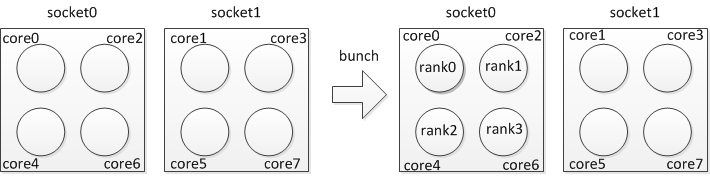
\includegraphics[width=0.9\columnwidth]{Img/nehalem-bunch.png}
 \caption{Process placement with ``bunch'' CPU binding policy}
 \label{fig:bunch}
\end{figure}

If you want to run 4 processes per node and utilize ``scatter'' policy on
each node, you can specify:

\CommandBox{\$ mpirun\_rsh -np 4 -hostfile hosts MV2\_CPU\_BINDING\_POLICY=scatter ./a.out}{0.9}

The CPU binding will be set as shown in Figure~\ref{fig:scatter}.

\begin{figure}[htbp]
 \centering
 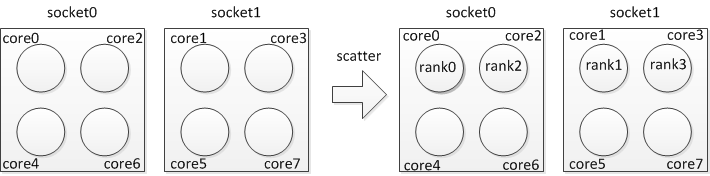
\includegraphics[width=0.9\textwidth]{Img/nehalem-scatter.png}
 \caption{Process placement with ``Scatter'' CPU binding policy}
 \label{fig:scatter}
\end{figure}

%If MV2\_ENABLE\_LEASTLOAD (Section \ref{def:mv2-enable-leastload})
%is set to 1,
%this scheme considers the current CPU load to set CPU
%binding with the binding
%policy.
%For example,
If two applications with four processes each need to share
a given node (with eight cores) at the same time with ``bunch'' policy, you
can specify:

\CommandBox{\$ mpirun\_rsh -np 4 -hostfile hosts MV2\_CPU\_BINDING\_POLICY=bunch ./a.out}{0.9}

\CommandBox{\$ mpirun\_rsh -np 4 -hostfile hosts MV2\_CPU\_BINDING\_POLICY=bunch ./b.out}{0.9}

The CPU binding will be set as shown in Figure~\ref{fig:bunch2}.

\begin{figure}[htbp]
 \centering
 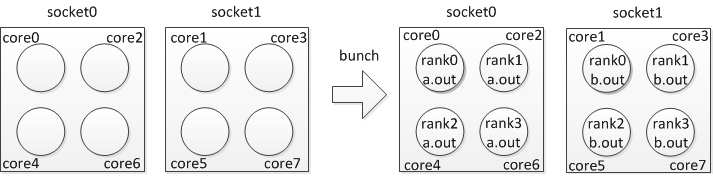
\includegraphics[width=0.9\textwidth]{Img/nehalem-bunch2.png}
 \caption{Process placement with two applications using the ``bunch'' CPU
			binding policy}
 \label{fig:bunch2}
\end{figure}

If two applications with four processes each need to share
a given node (with eight cores) at the same time
with ``scatter'' policy, you can specify:

\CommandBox{\$ mpirun\_rsh -np 4 -hostfile hosts MV2\_CPU\_BINDING\_POLICY=scatter ./a.out}{0.9}

\CommandBox{\$ mpirun\_rsh -np 4 -hostfile hosts MV2\_CPU\_BINDING\_POLICY=scatter ./b.out}{0.9}

The CPU binding will be set as shown in Figure~\ref{fig:scatter2}.

\begin{figure}[htbp]
 \centering
 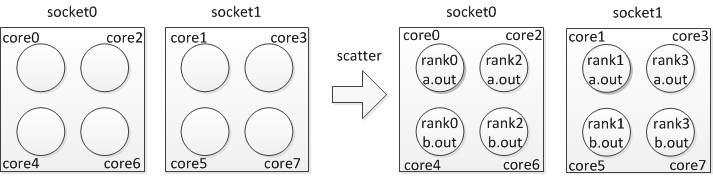
\includegraphics[width=0.9\textwidth]{Img/nehalem-scatter2.png}
 \caption{Process placement with two applications using the ``scatter'' CPU
			binding policy}
 \label{fig:scatter2}
\end{figure}

The aforementioned binding is based on the core level, meaning each MPI
process will be bound to a specific core. Actually, we provide different
process binding level. There are three binding levels: ``core'', ``socket'',
and ``numanode'' (which is designed for some multicore processor with NUMA
node unit). We use the ``core'' as the default binding level, and we
also allow users to choose a binding level through the run-time variable,
MV2\_CPU\_BINDING\_LEVEL. (Section \ref{def:mv2-cpu-binding-level})
For example, if you want to run 4 processes per node and utilize ``socket''
as the binding level on each node, you can specify:

\CommandBox{\$ mpirun\_rsh -np 4 -hostfile hosts MV2\_CPU\_BINDING\_LEVEL=socket ./a.out}{0.9}

The CPU binding will be set as shown in Figure~\ref{fig:socket_bunch}. Note:
because we use ``bunch'' as the default binding policy, all four processes will
be bound to the first socket and each of them can use all four cores in this
socket. When the binding policy is ``bunch'' and the binding level is
``socket'', processes will be bound to the same socket until the process number is
larger than the core number in the socket.

\begin{figure}[htbp]
 \centering
 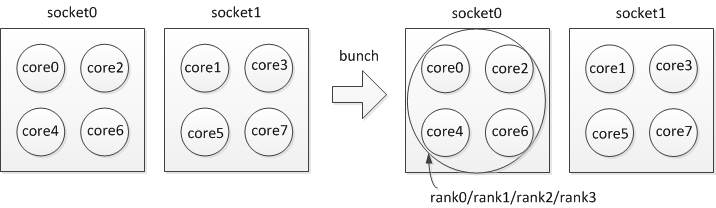
\includegraphics[width=0.9\textwidth]{Img/nehalem-socket-bunch.png}
 \caption{Process placement with the ``bunch'' CPU binding policy and
``socket'' binding level}
 \label{fig:socket_bunch}
\end{figure}

If you want to run 4 processes per node, utilize ``socket'' as the binding
level and ``scatter'' as the binding policy, you can specify:

\CommandBox{\$ mpirun\_rsh -np 4 -hostfile hosts MV2\_CPU\_BINDING\_LEVEL=socket MV2\_CPU\_BINDING\_POLICY=scatter ./a.out}{0.9}

The CPU binding will be set as shown in Figure~\ref{fig:socket_scatter}.

\begin{figure}[htbp]
 \centering
 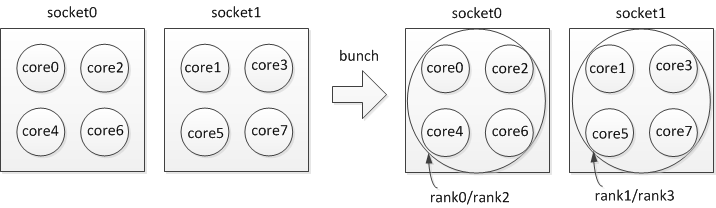
\includegraphics[width=0.9\textwidth]{Img/nehalem-socket-scatter.png}
 \caption{Process placement with the ``scatter'' CPU binding policy and
``socket'' binding level}
 \label{fig:socket_scatter}
\end{figure}


\subsubsection{Mapping Policies for Hybrid (MPI+Threads) Applications}
We have introduced one additional policy called ``hybrid" for
MV2\_CPU\_BINDING\_POLICY variable. This policy can also be used for hybrid
MPI+Threads (OpenMP, pthreads, etc.) applications where each MPI rank
additionally spawns multiple threads. The detailed usage of this variable and
any additional variables you might need is discussed in
Section~\ref{sec:knl_multi_thread}.

In addition to MV2\_CPU\_BINDING\_POLICY, we have also provided a new
environment variable called MV2\_HYBRID\_BINDING\_POLICY to specify thread
specific binding policies. The detailed description and usage of this variable
is explained in Section~\ref{sec:advanced_thread_binding_policies}.

\subsubsection{User defined CPU Mapping}
\label{usage:mv2_cpu_mapping}
Under the second scheme, users can also use
their own mapping to bind processes to  CPU's on modern
multi-core systems.  The feature is especially useful
on multi-core systems, where performance may be different if processes are
mapped to
different cores. The mapping can be specified by setting the environment
variable
\texttt{MV2\_CPU\_MAPPING} (Section ~\ref{def:mv2-cpu-mapping}).

For example, if you want to run 4 processes per node and utilize cores
0, 1, 4, 5 on each node, you can specify:

\CommandBox{\$ mpirun\_rsh -np 64 -hostfile hosts MV2\_CPU\_MAPPING=0:1:4:5
./a.out}{0.9}

or

\CommandBox{\$ mpiexec -n 64 -f hosts -env MV2\_CPU\_MAPPING 0:1:4:5 ./a.out}{0.9}

In this way, process 0 on each node will be mapped to core 0, process 1 will be
mapped to
core 1, process 2 will be mapped to core 4, and process 3 will be mapped to core
5.
For each process, the mapping is separated by a single ``:".

MVAPICH2 supports binding one process to multiple cores in the same node with ``," or ``-". For example:

\CommandBox{\$ mpirun\_rsh -np 64 -hostfile hosts MV2\_CPU\_MAPPING=0,2,3,4:1:5:6
./a.out}{0.9}

or

\CommandBox{\$ mpirun\_rsh -np 64 -hostfile hosts MV2\_CPU\_MAPPING=0,2-4:1:5:6
./a.out}{0.9}

In this way, process 0 on each node will be mapped to core 0, core 2, core 3, and core 4; process 1 will
be mapped to core 1, process 2 will be mapped to core 5, and process 3 will be mapped to core 6.
This feature is designed to support the case that one rank process will spawn multiple threads and set
thread binding in the program.

\subsubsection{Performance Impact of CPU Mapping}
\label{usage:perf_cpu_mapping}
Here we provide a table with latency performance of 0 byte and 8KB messages
using different CPU mapping schemes. The results show how process binding can
affect the benchmark performance. We strongly suggest the consideration of
best CPU
mapping on multi-core platforms
when carrying out benchmarking and performance evaluation with
MVAPICH2.

The following measurements were taken on the machine with the dual quad-core
2.53GHz Intel Xeon processors with 12MB L3 shared cache (among cores in one
socket). MVAPICH2-\mvapichrcversion was
built with gcc-4.4.6 and default configure arguments:

\begin{table*}[h]
%\begin{center}
\begin{tabular}{|l*{3}{|l}|}
\hline
&\multicolumn{2}{|c|}{Message Latency}&\\
\cline {2-3}
Core Pair&0-byte&8k-byte&\multicolumn{1}{|c|}{Notes}\\
\hline
1,2&0.17 us&1.83 us&same socket, shared L3 cache, best performance\\
\hline
0,1&0.17 us&1.87 us&same socket, shared L3 cache, but core 0 handles interrupts\\
\hline
1,5&0.41 us&3.16 us&different sockets\\
\hline
0,4&0.42 us&3.17 us&different sockets, but core 0 handles interrupts\\
\hline
\end{tabular}
%\end{center}
\label{table:cpumapping_perf}
\end{table*}

%PLPA supports more flexible notations
%when specifying core mapping. More details
%can be
%found at:

%\texttt{http://www.open-mpi.org/community/lists/plpa-users/2007/04/0035.php}

%To take advantage of any of these features, the jobs need to run with CPU
%affinity turned on (default). If users choose to set
%MV2\_ENABLE\_AFFINITY to 0, then the kernel takes care of mapping processes to
%cores and none of the above features will be enabled. More details about using
%this parameter can be found in Section \ref{def:mv2-cpu-mapping}.






\subsection{Running with LiMIC2}
\label{usage:mv2-limic2}

MVAPICH2 CH3-based interfaces support LiMIC2 for intra-node communication for medium and large
messages to get higher performance. LiMIC2 is also used to optimize intra-node one-sided communication in
OFA-IB-CH3 and OFA-iWARP-CH3 interfaces. It is disabled by default because it depends on the LiMIC2
package to be previously installed. As a convenience we have distributed the latest LiMIC2 package (as of this release)
with our sources.

To install this package, please take the following steps.

\begin{itemize}
\item Navigate to the LiMIC2 to source\\
        \CommandBox{\$ cd limic2-0.5.6}{0.9}

\item Configure and build the source\\
        \CommandBox{limic2-0.5.6\$ ./configure --enable-module
            --prefix=/usr --sysconfdir=/etc \&\& make}{0.9}

\item Install\\
        \CommandBox{limic2-0.5.6\$ sudo make install}{0.9}
\end{itemize}

Before using LiMIC2 you'll need to load the kernel module.  If you followed the
instructions above you can do this using the following command (LSB init
script).

\begin{itemize}
\item \CommandBox{\$ /etc/init.d/limic start}{0.9}
\end{itemize}

Please note that supplying `\texttt{--sysconfdir=/etc}' in the configure line
above told the package to install the init script and an udev rule in the
standard location for system packages.  Supplying `\texttt{--prefix=/usr}' will
also install the headers and libraries in the system path.  These are optional
but recommended.

Now you can use LiMIC2 with MVAPICH2 by simply supplying the
`\texttt{--with-limic2}' option when configuring MVAPICH2.  You can run your
applications as normal and LiMIC2 will be used by default. To disable it at run time,
use the env variable:

\CommandBox{\$ mpirun\_rsh -np 64 -hostfile hosts MV2\_SMP\_USE\_LIMIC2=0 ./a.out}{0.9}

\subsection{Running with Shared Memory Collectives}

In MVAPICH2, support for shared memory based collectives has
been enabled for MPI applications running over OFA-IB-CH3,
OFA-iWARP-CH3, TrueScale (PSM-CH3) and Omni-Path (PSM2-CH3) interfaces.  Currently,
this support is available for the following
collective operations:
\begin{itemize}
		\item{MPI\_Allreduce}
		\item{MPI\_Reduce}
		\item{MPI\_Barrier}
		\item{MPI\_Bcast}
\end{itemize}

Optionally, these feature can be turned off at run time by using the
following parameters:
\begin{itemize}
	\item{\texttt{MV2\_USE\_SHMEM\_COLL} (section~\ref{def:mv2-use-shmem-coll}})
			
		\item{\texttt{MV2\_USE\_SHMEM\_ALLREDUCE} (section~\ref{def:mv2-use-shmem-allreduce}})

		\item{\texttt{MV2\_USE\_SHMEM\_REDUCE} (section~\ref{def:mv2-use-shmem-reduce}})
		
		\item{\texttt{MV2\_USE\_SHMEM\_BARRIER} (section~\ref{def:mv2-use-shmem-barrier}})
		\item{\texttt{MV2\_USE\_SHMEM\_BCAST} (section~\ref{def:mv2-use-shmem-bcast}})
			\end{itemize}

Please refer to Section~\ref{def:mvapich-parameters} for further details.

\subsection{Running with Topology-Aware Shared Memory Collectives}

In MVAPICH2, support for intra-node topology aware collectives is enabled by default. This feature can be toggled using
MV2\_ENABLE\_TOPO\_AWARE\_COLLECTIVES (section~\ref{def:mv2-enable-socket-aware-collectives}). It requires shared
memory collectives to be enabled (section ~\ref{def:mv2-use-shmem-coll}). Supported interfaces include 
OFA-IB-CH3, OFA-iWARP-CH3, TrueScale (PSM-CH3) and Omni-Path (PSM2-CH3). Currently,
this support is available for the following collective operations:
\begin{itemize}
                \item{MPI\_Allreduce}
                \item{MPI\_Barrier}
\end{itemize}

Run-time parameters exist to toggle each one of the supported collective operations. The parameters are :
\begin{itemize}
\item{\texttt{MV2\_USE\_TOPO\_AWARE\_ALLREDUCE} (section~\ref{def:mv2-use-topo-aware-allreduce}})
\item{\texttt{MV2\_USE\_TOPO\_AWARE\_BARRIER} (section~\ref{def:mv2-use-topo-aware-barrier}})
\end{itemize}

MVAPICH2 also provides support for topology-aware allreduce with SHArP support
for inter-node operations by default. Please refer to
Section~\ref{subsec:coll-sharp} for more details on how to enable this feature.

Please refer to Section~\ref{def:mvapich-parameters} for further details.

\subsection{Running Collectives with Hardware based Multicast support}
\label{subsec:coll-mcast}

In MVAPICH2, support for multicast based collectives has
been enabled for MPI applications running over OFA-IB-CH3 interface.
Currently, this support is available for the following
collective operations:

\begin{itemize}
		\item{MPI\_Bcast}
		\item{MPI\_Allreduce}
		\item{MPI\_Scatter}
\end{itemize}

This feature is enabled by default. This can be toggled at runtime by using
parameter \\
MV2\_USE\_MCAST (section~\ref{def:use-mcast}).  This feature is effective when the MPI job is running on
more than the threshold \\
MV2\_MCAST\_NUM\_NODES\_THRESHOLD (section~\ref{def:mcast-num-nodes-thrshold})
number of nodes.

Both RDMA\_CM and libibumad based multicast group setup schemes are supported.

RDMA\_CM based multicast group setup (enabled by default) can be toggled using
the \\ MV2\_USE\_RDMA\_CM\_MCAST (section~\ref{def:mv2-use-rdma-cm-mcast}) run-time parameter.

If RDMA\_CM based mutlicast group setup is disabled/cannot be used, multicast requires the cluster to be installed with 
libibumad and libibmad libraries as well as have read/write permission for users on /dev/infiniband/umad0 to function properly.

If neither RDMA\_CM nor libibumad based group setup for multicast are viable options, then the feature can be disabled using the --disable-mcast configure flag.
\begin{verbatim}
$ ls -l /dev/infiniband/umad0
crw-rw-rw- 1 root root 231, 0 Jul  8 19:47 /dev/infiniband/umad0
\end{verbatim}

\subsection{Running MPI\_Gather collective with intra-node Zero-Copy  designs (using LiMIC2)}
\label{subsec:coll-mcast}
In MVAPICH2, we offer new intra-node Zero-Copy designs (using LiMIC2) for the MPI\_Gather collective operation based
on the LiMIC2 feature. This feature can be used, when the library has been
configured to use LiMIC2(~\ref{usage:mv2-limic2}). This feature is disabled by
default and can be turned on at runtime by using the parameter
MV2\_USE\_LIMIC\_GATHER (~\ref{def:use-limic-gather}).

\subsection{Running with scalable UD transport}
\label{subsec:mpi-ud}
MVAPICH2 has scalable design with InfiniBand connection less transport
Unreliable Datagram (UD). Applications can use UD only transport by
simply configuring MVAPICH2 with the ‘--enable-hybrid’ (which is enabled
by default) and setting the environment 
variable MV2\_USE\_ONLY\_UD (~\ref{def:use-only-ud}).
In this mode, library does not use any reliable RC connections.
This feature eliminates all the overheads associated with RC connections
and reduces the memory footprint at large scale.

\subsection{Running with Integrated Hybrid UD-RC/XRC design}
\label{subsec:mpi-hybrid}
MVAPICH2 has integrated hybrid transport support for OFA-IB-CH3.
This provides the capability to use Unreliable Datagram (UD),
Reliable Connection (RC) and eXtended Reliable Connection (XRC)
transports of InfiniBand. This hybrid transport design is targeted at emerging
clusters with multi-thousand core clusters to deliver best possible
performance and scalability with constant memory footprint.

Applications can use Hybrid transport by simply configuring MVAPICH2
with the ‘--enable-hybrid’ option.  In this configuration, MVAPICH2
seamlessly uses UD and RC/XRC connections by default. The use of UD
transport can be disabled at run time by setting the environment variable
MV2\_USE\_UD\_HYBRID(~\ref{def:use-ud-hybrid}) to Zero.

MV2\_HYBRID\_ENABLE\_THRESHOLD (~\ref{def:ud-hybrid-threshold})
defines the threshold for enabling the hybrid transport.
Hybrid mode will be used when the size of the job is greater than
or equal to the threshold. Otherwise, it uses default RC/XRC connections.

%For a full list of Hybrid environment variables, please refer to the section ~\ref{def:mvapich-ud-hybrid}.
For a full list of Hybrid environment variables, please refer Section~\ref{def:mvapich-parameters}.

\subsection{Running with Multiple-Rail Configurations}
\label{subsec:mpi-mr}

MVAPICH2 has integrated multi-rail support for OFA-IB-CH3 and
OFA-iWARP-CH3 interfaces. Run-time variables are used to specify the
control parameters of the multi-rail support; number of adapters with
MV2\_NUM\_HCAS (section~\ref{def:num-hcas}), number of ports per adapter
with MV2\_NUM\_PORTS (section~\ref{def:num-ports}), and number of queue
pairs per port with MV2\_NUM\_QP\_PER\_PORT
(section~\ref{def:num-qp-per-port}). Those variables are default to 1 if
you do not specify them.

Large messages are striped across all HCAs. The threshold for striping
is set according to the following formula: \\
(MV2\_VBUF\_TOTAL\_SIZE $\times$ MV2\_NUM\_PORTS $\times$
MV2\_NUM\_QP\_PER\_PORT $\times$
MV2\_NUM\_HCAS). In addition, there is another parameter
MV2\_STRIPING\_THRESHOLD (section~\ref{def:viadev-striping-threshold}) which users can
utilize to set the striping threshold directly.

MVAPICH2 also gives the flexibility to balance short message traffic over
multiple HCAs in a multi-rail configuration. The run-time variable
MV2\_SM\_SCHEDULING can be used to choose between the various load balancing
options available. It can be set to USE\_FIRST (Default) or ROUND\_ROBIN. In
the USE\_FIRST scheme, the HCA in slot 0 is always used to transmit
the short messages. If ROUND\_ROBIN is chosen, messages are sent across all
HCAs alternately.

In the following example, we can use multi-rail support with two
adapters, using one port per adapter and one queue pair per port:\\

\CommandBox{\$ mpirun\_rsh -np 2 n0 n1 MV2\_NUM\_HCAS=2 MV2\_NUM\_PORTS=1
MV2\_NUM\_QP\_PER\_PORT=1 prog}{0.9}\\

Using the Hydra process manager, the same can be accomplished by:\\

\CommandBox{\$ mpiexec -n 2 -hosts n0,n1 -env MV2\_NUM\_HCAS 2 -env
MV2\_NUM\_PORTS 1 -env MV2\_NUM\_QP\_PER\_PORT 1 prog}{0.9}\\
\\

Note that the default values of \texttt{MV2\_NUM\_PORTS} and
\texttt{MV2\_NUM\_QP\_PER\_PORT} are 1, so they can be omitted.

\CommandBox{\$ mpirun\_rsh -np 2 n0 n1 MV2\_NUM\_HCAS=2 prog}{0.9}\\

Using the Hydra process launcher, the following command can be used:\\

\CommandBox{\$ mpiexec -n 2 -hosts n0,n1 -env MV2\_NUM\_HCAS 2 prog}{0.9}

The user can also select the particular network card(s) that should be
used by using the MV2\_IBA\_HCA environment variable specified
in section~\ref{def:rdma-iba-hcas}. The following is an example of how to run
MVAPICH2 in this mode. (In the example ``mlx4\_0'' is the name of the
InfiniBand card as displayed by the output of the ``ibstat'' command).

\CommandBox{\$ mpirun\_rsh -np 2 n0 n1 MV2\_IBA\_HCA=mlx4\_0 prog}{0.9}\\

If there are multiple HCAs in the system, the user can also selectively
use some or all of these HCAs for network operations by using the
MV2\_IBA\_HCA environment variable. Different HCAs are delimited by
colons ``:''. An example is shown below. In the example ``mlx4\_0'' and
``mlx4\_1'' are the names of the InfiniBand card as displayed by the
output of the ``ibstat'' command. There can be other HCAs in the system
as well.

\CommandBox{\$ mpirun\_rsh -np 2 n0 n1 MV2\_IBA\_HCA=mlx4\_0:mlx4\_1 prog}{0.9}\\

\subsection{Enhanced design for Multiple-Rail Configurations}
\label{subsec:mpi-mr_new}
MVAPICH2 now features an enhanced design for multiple rail
configurations for OFA-IB-CH3 and OFA-iWARP-CH3 interfaces. It can
broadly be explained by the figure given below. In addition to the
earlier design where the rails were shared among processes at run time
(as depicted under the Rail Sharing banner in the figure below),
MVAPICH2 now features a new RAIL BINDING policy which will dedicate a
particular rail to a particular process.

\begin{figure}[htbp]
 \centering
 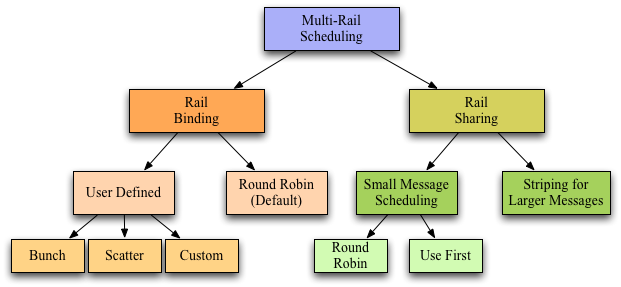
\includegraphics[width=0.9\textwidth]{Img/multi-rail-design.png}
 \caption{Multi-rail Scheduling policies}
 \label{fig:mrail_new}
\end{figure}

The scheduling policies are broadly classified into 2 basic types.
Rail Binding and Rail Sharing.

\begin{itemize}
    \item The Rail Sharing policy has been kept the same as in earlier
          versions and can be set using the MV2\_RAIL\_SHARING\_POLICY
          (section~\ref{def:rail-sharing-policy})
          (previously MV2\_SM\_SCHEDULING) parameter. It can take the
          values USE\_FIRST or ROUND\_ROBIN. However as opposed to the
          earlier versions, the number of HCAs of the same type on a
          system get detected automatically and used. The user can still
          make use of the MV2\_NUM\_HCAS parameter and set the number to
          a custom number of rails if required. If this parameter is not
          set the maximum number gets used.
    \item In the Rail Binding policy only that HCAs is made available to
          the process which has been assigned to it using some scheme. The
          default policy used is 'Rail Binding in a round-robin manner': If
          the parameter MV2\_RAIL\_SHARING\_POLICY is not specified, MVAPICH2
          assigns HCAs to the processes in a round-robin manner. The Rail
          Binding policy can either be default as described above or user defined.
          For the user defined mode the following parameter
          MV2\_RAIL\_SHARING\_POLICY=FIXED\_MAPPING should be set.

          The user defined policies can be set in the following manner by giving
          appropriate values to the parameter MV2\_PROCESS\_TO\_RAIL\_MAPPING
          (section~\ref{def:process-to-rail-mapping})

          \begin{itemize}
              \item MV2\_PROCESS\_TO\_RAIL\_MAPPING=BUNCH : The HCAs are assigned in a
                    block manner. e.g. For 4 rails and 16 processes the mapping
                    will be – 0:0:0:0:1:1:1:1:2:2:2:2:3:3:3:3
              \item MV2\_PROCESS\_TO\_RAIL\_MAPPING=SCATTER : The HCAs are assigned
                    in a cyclic manner. e.g. For 4 rails and 16 processes the mapping
                    will be – 0:1:2:3:0:1:2:3:0:1:2:3:0:1:2:3
              \item The third option is a custom list which can be passed as a string
                    to \\ MV2\_PROCESS\_TO\_RAIL\_MAPPING separated by a colon(:) as shown above.
          \end{itemize}
    \item In addition to these parameters the other ENVS that can be set are
          MV2\_VBUF\_TOTAL\_SIZE, \\ MV2\_NUM\_QP\_PER\_PORT,
          MV2\_RAIL\_SHARING\_LARGE\_MSG\_THRESHOLD \\ (previously MV2\_STRIPING\_THRESHOLD),
          MV2\_IBA\_HCA. Please refer to the usage described for these parameters as well as
          the ones described above in (section~	\ref{def:mvapich-parameters}).
\end{itemize}

\begin{comment}
\subsection{Running with QoS enabled Configurations}
\label{subsec:mpi-qos}

MVAPICH2 allows the user to load balance messages over multiple virtual
lanes in a QoS configuration for OFA-IB-CH3 interface. The run-time
variable MV2\_NUM\_SLS can be used to choose the number service levels
the user wants the MVAPICH2 library to use to load balance traffic. The
assumption is that each service level is mapped to a different virtual
lane and that all virtual lanes have equal priority. This configuration
needs to be performed by the system administrator through OpenSM.
Currently MVAPICH2 only supports distributing traffic evenly across all
the service levels (and in turn virtual lanes).

Following is an example to run MVAPICH2 with multiple service levels:

\CommandBox{\$ mpirun\_rsh -np 2 n0 n1 MV2\_NUM\_SLS=4 prog}{0.9}\\

    \subsubsection{How to enable and verify QoS in an IB system}
    \label{subsubsec:enabling-qos}

    The steps required to enable QoS in an IB system are as follows

    \begin{itemize}

        \item{Create a QoS config file. Figure~\ref{fig:qos_config} shows a
              sample QoS configuration file}
        \item{Restart OpenSM in a QoS mode such that it
              uses and honors the contents of this file
              eg: opensm~-Q~-Y~$<$Path~to~qos~config~file$>$}
        \item{Add the following line to /etc/modprobe.conf file
              "options mlx4\_core enable\_qos=1"}
        \item{Either re-load the IB drivers or reboot the system}

    \end{itemize}

    The command \textit{smpquery} can be used to retrieve information relating
    to QoS (among others) from the InfiniBand fabric.

    smpquery $<$sl2vl\/vlarb$>$ $<$lid$>$ $<$port$>$

    \begin{figure}
    \begin{verbatim}

    [root@n0 ~]# /usr/sbin/smpquery sl2vl 1 0
    # SL2VL table: Lid 1
    #                 SL: | 0| 1| 2| 3| 4| 5| 6| 7| 8| 9|10|11|12|13|14|15|
    ports: in  0, out  0: | 0| 1| 2| 3| 4| 5| 6| 7|15|15|15|15|15|15|15| 7|

    [root@n0 ~]# /usr/sbin/smpquery vlarb 1 0
    # VLArbitration tables: Lid 1 port 0 LowCap 8 HighCap 8
    # Low priority VL Arbitration Table:
    VL    : |0x0 |0x1 |0x2 |0x3 |0x4 |0x5 |0x6 |0x7 |
    WEIGHT: |0x14|0x14|0x14|0x14|0x14|0x14|0x14|0x14|
    # High priority VL Arbitration Table:
    VL    : |0x0 |0x1 |0x2 |0x3 |0x4 |0x5 |0x6 |0x7 |
    WEIGHT: |0xA |0xA |0xA |0xA |0xA |0xA |0xA |0xA |

    \end{verbatim}
    \caption{Sample Output from \textit{smpquery} command}
    \label{fig:smp_query}
    \end{figure}

    \begin{figure}
    \begin{verbatim}

    # QoS config to setup SL to VL mappings

    #Max number of VL's that a CA in this subnet can support
        qos_ca_max_vls 8

    #Max number of packets VL's in the VLArb_High table may send before yielding
    #to VL's in VLArb_Low table. The number of bytes that can be sent is
    #qos_<type>_high_limit * 4KB(MTU).
        qos_ca_high_limit 255

    #VL:Number of 64 byte units the HCA may send through this VL when its turn comes
    #One 64 byte unit needs 1 credit to transfer.
        qos_ca_vlarb_high 0:255
        qos_ca_vlarb_high 0:10,1:10,2:10,3:10,4:10,5:10,6:10,7:10
        qos_ca_vlarb_low 0:20,1:20,2:20,3:20,4:20,5:20,6:20,7:20

    #SL2VL Mapping for Host Channel Adapters
        qos_ca_sl2vl 0,1,2,3,4,5,6,7,15,15,15,15,15,15,15,15

    #Max number of VL's that a switch in this subnet can support
        qos_swe_max_vls 8
        qos_swe_high_limit 255

    #VL:Number of 64 byte units the switch may send through this VL when its turn comes
    #One 64 byte unit needs 1 credit to transfer.
        qos_swe_vlarb_high 0:10,1:10,2:10,3:10,4:10,5:10,6:10,7:10
        qos_swe_vlarb_low 0:20,1:20,2:20,3:20,4:20,5:20,6:20,7:20

    #SL2VL Mapping for Switches
        qos_swe_sl2vl 0,1,2,3,4,5,6,7,15,15,15,15,15,15,15,15

    \end{verbatim}
    \caption{Sample QoS Configuration File}
    \label{fig:qos_config}
    \end{figure}
\end{comment}

\subsection{Running with Fault-Tolerance Support}
\label{subsec:mpi-ft}

\subsubsection{System-Level Checkpoint/Restart}
\label{subsubsec:mpi-cr}

MVAPICH2 provides system-level rollback-recovery capability based on a
coordinated Checkpoint-Restart protocol involving all the application processes.

The following section (~\ref{para:mpi-cr-basic}) provides instructions for basic
checkpoint/restart operations with MVAPICH2. These require the Berkeley Lab
Checkpoint/Restart (BLCR) library in order perform checkpoints of local
processes. Then, advanced features are presented.
Section~\ref{para:mpi-cr-aggr} details the usage of the fast-checkpointing
scheme based on aggregation.  Section~\ref{para:mpi-cr-ftb} present the support
of the new standardized Fault Tolerance Backplane (FTB).

\paragraph{Basic Checkpoint/Restart Scheme:}
\label{para:mpi-cr-basic}

BLCR is a library that allows to take checkpoint of individual processes.  Its
usage is mandatory to take advantage of the checkpoint/restart functionality in
MVAPICH2.  Here are the steps that allows the usage of BLCR with MVAPICH2.

\begin{itemize}
  \item Download and install the BLCR (Berkeley Lab's
    Checkpoint/Restart) package. The packages can be
    downloaded from
    \href{http://crd.lbl.gov/groups-depts/ftg/projects/current-projects/BLCR/berkeley-lab-checkpoint-restart-for-linux-blcr-downloads/}
    {this web page}.

  \item Make sure the BLCR packages are installed on every node
    and the \texttt{LD\_LIBRARY\_PATH} must contain the path
    to the shared library of BLCR, usually
    \texttt{\${BLCR\_HOME}/lib}.

  \item MVAPICH2 needs to be compiled with checkpoint/restart support, see
    section~\ref{subsec:config-gen2}.

  \item BLCR kernel modules must be loaded on all the compute nodes.

  \item Make sure the PATH contains the path to the executables of
    BLCR, usually \texttt{\${BLCR\_HOME}/bin}.
\end{itemize}

Users are strongly encouraged to read the
\href{http://upc-bugs.lbl.gov/blcr/doc/html/BLCR\_Admin\_Guide.html}{Administrators
guide} of BLCR, and test the BLCR on the target platform, before using the
checkpointing feature of MVAPICH2.

\noindent\textbf{Checkpointing operation}\\

Now, your system is set up to use the Checkpoint/Restart features of MVAPICH2.
Several parameters are provided by MVAPICH2 for flexibility in configuration and
using the Checkpoint / Restart features. If mpiexec is used as the job start up
mechanism, these parameters need to be set in the user's environment through the
BASH shell's \texttt{export} command, or the equivalent command for other
shells. If mpirun\_rsh is used as the job start up mechanism, these parameters
need to be passed to mpirun\_rsh through the command line.

\begin{itemize}
  \item{MV2\_CKPT\_FILE}: This parameter specifies the path and
    the base file name for checkpoint files of MPI processes.
    Please note that File System performance is critical to
    the performance of checkpointing. This parameter
    controls which file system will be used to store the
    checkpoint files. For example, if your PVFS2 is mounted
    at\\ \texttt{/mnt/pvfs2}, using \texttt{
    MV2\_CKPT\_FILE=/mnt/pvfs2/ckptfile} will let the
    checkpoint files being stored in pvfs2 file system. See
    Section~\ref{def:mv2-ckpt-file} for details.

  \item{MV2\_CKPT\_INTERVAL}: This parameter (in minutes) can be used to
    enable automatic checkpointing. See
    Section~\ref{def:mv2-ckpt-interval} for details.

  \item{MV2\_CKPT\_MAX\_SAVE\_CKPTS}: This parameter is used to
    limit the number of checkpoints saved on file system.
    See Section~\ref{def:mv2-max-save-ckpts} for details.

  \item{MV2\_CKPT\_NO\_SYNC}: This parameter is used to control
    whether the program forces the checkpoint files being
    synced to disk or not before it continues execution.
    See Section~\ref{def:mv2-ckpt-no-sync} for details.

\end{itemize}

In order to provide maximum flexibility to end users who wish to use the
checkpoint/restart features of MVAPICH2, we have provided three different
methods that can be used to take checkpoints during the execution of the MPI
application. These methods are described as follows:

\begin{itemize}
    \item Manual Checkpointing: In this mode, the user simply launches an MPI
    application and chooses when to checkpoint the application. This mode can be
    primarily used for experimentation during deployment stages. In order to use
    this mode, the MPI application is launched normally using \texttt{mpiexec}
    or \texttt{mpirun\_rsh}.  When the user decides to take a checkpoint, the
    users can issue a BLCR command namely ``\texttt{cr\_checkpoint}'' in the
    following manner:

    \begin{verbatim} cr_checkpoint -p <PID> \end{verbatim}

    where PID is the process id of the \texttt{mpiexec} or \texttt{mpirun\_rsh}
    process. In order to simplify the process, the script
    \texttt{mv2\_checkpoint} can be used. This script is available in the same
    directory as \texttt{mpiexec} and \texttt{mpirun\_rsh}.

    \item Automated Checkpointing: In this mode, the user can launch the MPI
    application normally using \texttt{mpiexec} or \texttt{mpirun\_rsh}.
    However, instead of manually issuing checkpoints as described in the above
    bullet, a parameter (\texttt{MV2\_CKPT\_INTERVAL}) can be set to
    automatically take checkpoints and user-defined intervals. Please refer to
    Section~\ref{def:mv2-ckpt-interval} for a complete usage description of this
    variable. This mode can be used to take checkpoints of a long running
    application, for example every 1 hour, 2 hours etc. based on user's choice.

    \item Application Initiated Synchronous Checkpointing: In this mode, the MPI
    application which is running can itself request for a checkpoint.
    Application can request a whole program checkpoint synchronously by calling
    \texttt{MVAPICH2\_Sync\_Checkpoint}. Note that it is a collective operation,
    and this function must be called from all processes to take the checkpoint.
    This mode is expected to be used by applications that can be modified and
    have well defined synchronization points. These points can be effectively
    used to take checkpoints. An example of how this mode can be activated is
    given below.

    \begin{verbatim}
    #include "mpi.h"
    #include <unistd.h>
    #include <stdio.h>

    int main(int argc,char *argv[])
    {
        MPI_Init(&argc,&argv);
        printf("Computation\n");
        sleep(5);
        MPI_Barrier(MPI_COMM_WORLD);
        MVAPICH2_Sync_Checkpoint();
        MPI_Barrier(MPI_COMM_WORLD);
        printf("Computation\n");
        sleep(5);
        MPI_Finalize();
        return 0;
    }
    \end{verbatim}

\end{itemize}

\noindent\textbf{Restart operation}

To restart a job from a \textbf{manual checkpoint}, users need to issue another
command of BLCR, ``\texttt{cr\_restart}'' with the checkpoint file name of the
MPI job console as the parameter. Usually, this file is named
\\\texttt{context.$<$pid$>$}. The checkpoint file name of the MPI job console
can be specified when issuing the checkpoint (see the ``\texttt{cr\_checkpoint
--help}'' for more information). Please note that the names of checkpoint files
of the MPI processes will be assigned according to the environment variable
{MV2\_CKPT\_FILE}, \\(\texttt{\${MV2\_CKPT\_FILE.$<$number of
checkpoint$>$.$<$process rank$>$}}).

To restart a job from an \textbf{automatic checkpoint}, use \texttt{cr\_restart
\$MV2\_CKPT\_FILE.$<$number of checkpoint$>$.auto}.

If the user wishes to restart the MPI job on a different set of nodes, the host
file that was specified along with the ``\texttt{-hostfile}" option during job
launch phase should be modified accordingly before trying to restart a job with
``\texttt{cr\_restart}''. This modified ``\texttt{hostfile}" must be at the same
location and with the same file name as the original hostfile.  The mpirun\_rsh
framework parses the host file again when trying to restart from a checkpoint,
and launches the job on the corresponding nodes. This is possible as long as the
nodes in which the user is trying to restart has the exact same environment as
the one in which the checkpoint was taken (including shared NFS mounts, kernel
versions, and user libraries).

For this to function correctly, the user should disable pre-linking on both the
source and the destination node.  See the
~\href{https://upc-bugs.lbl.gov//blcr/doc/html/FAQ.html#prelink}{FAQ Section} of
the BLCR userguide for more information.

Please refer to the Section~\ref{sec:troubleshooting-ckpt} for troubleshooting
with Checkpoint/Restart.

\paragraph{Write-Aggregation based Fast Checkpointing Scheme:}
\label{para:mpi-cr-aggr}

MVAPICH2 provides an enhanced technique that allows fast checkpoint and restart.
This scheme, named Aggregation, relies on the Filesystem in Userspace (FUSE)
library.

Although Aggregation is optional, its usage is recommended to achieve best
performances during checkpoint and restart operations. That is why, if the FUSE
library is detected during configuration step, it will be automatically enabled
(see section~\ref{subsec:config-gen2}). Once enabled at configuration step,
aggregation scheme can be disabled at run time by setting the environment
variable \texttt{MV2\_CKPT\_USE\_AGGREGATION=0} (see
section~\ref{def:mv2-ckpt-use-aggregation} for details).


The following steps need to be done to use FUSE library for aggregation scheme.

\begin{itemize}
    \item Download and install the Filesystem in Userspace (FUSE) library
    package. The packages can be downloaded from
    \href{http://fuse.sourceforge.net/}{this web page}.  To get the best
    performance, users are encouraged to upgrade to kernel version $\geq 2.6.26$
    and use FUSE library $\geq 2.8$.

    \item Make sure the FUSE packages are installed on every node and the
    \texttt{LD\_LIBRARY\_PATH} must contain the path to the shared library of
    FUSE, usually \texttt{\${FUSE\_HOME}/lib}.

    \item MVAPICH2 needs to be compiled with checkpoint/restart support, see
    section~\ref{subsec:config-gen2}.

    \item FUSE kernel modules must be loaded on all the compute nodes.

    \item Make sure the PATH contains the path to the executables of FUSE,
    usually \texttt{\${FUSE\_HOME}/bin}.
\end{itemize}

If write aggregation has been enabled at configuration time, MVAPICH2 will
check the FUSE configuration of each node during startup (FUSE module loaded
and \texttt{fusermount} command in the PATH). If one node is not properly
configured, then MVAPICH2 will abort. In this case, you need to fix the FUSE
configuration of the nodes, or disable aggregation using
\texttt{MV2\_CKPT\_USE\_AGGREGATION=0} to run MVAPICH2.


\paragraph{Fault Tolerance Backplane (FTB) support:}
\label{para:mpi-cr-ftb}

MVAPICH2 supports the new standardized Fault Tolerance Backplane (FTB).  FTB can
be used for Checkpoint-Restart and Job Pause-Migration-Restart Frameworks.
Activating FTB support is optional to perform checkpoint/restart operations, but
it will allow MVAPICH2 to automatically publish and listen to standardized
events through the Fault Tolerance Backplane.


FTB has been developed and standardized by the
\href{http://www.mcs.anl.gov/research/cifts/}{CIFTS project}.  It enables faults
to be handled in a coordinated and holistic manner in the entire system,
providing for an infrastructure which can be used by different software systems
to exchange fault-related information.

If using the FTB framework for checkpoint/restart, the following steps need to
be done in addition to the above nodes.

\begin{itemize}

    \item Download and install the FTB (Fault Tolerance Backplane) package. The
    packages can be downloaded from
    \href{https://github.com/codes-org/codes/releases}{here}.

    \item Make sure the FTB packages are installed on every node and the
    \texttt{LD\_LIBRARY\_PATH} must contain the path to the shared library of
    FTB, usually \texttt{\${FTB\_HOME}/lib}.

    \item MVAPICH2 needs to be compiled with checkpoint/restart as well as FTB
    support, see section~\ref{subsec:config-gen2}.

    \item Start FTB Database server
    (\texttt{\${FTB\_HOME}/sbin/ftb\_database\_server}) on one of the nodes,
    this node will act as server node for all the FTB agents.

	\item Start FTB agents (\texttt{\${FTB\_HOME}/sbin/ftb\_agent}) on all the compute nodes.

\end{itemize}

\paragraph{Checkpoint/Restart support for the OFA-IB-Nemesis Interface:}
\label{para:mpi-cr-nem}

MVAPICH2 also provides Checkpoint-Restart capabilities for the OFA-IB-Nemesis
interface.  Currently, this feature can only be used in conjunction with the
Hydra process manager.  More details on using Hydra to checkpoint an MPI
application can be
found~\href{http://wiki.mcs.anl.gov/mpich2/index.php/Using_the_Hydra_Process_Manager#Checkpoint.2FRestart_Support}{here}.

\subsubsection{Multi-Level Checkpointing with Scalable Checkpoint-Restart\,(SCR)}
\label{subsubsec:checkpoint-scr}

The ~\href{https://computing.llnl.gov/projects/scalable-checkpoint-restart-for-mpi}{Scalable
Checkpoint-Restart}\,(SCR) library developed at the Lawrence Livermore National
Laboratory\,(LLNL) enables MPI applications to utilize distributed storage on
Linux clusters to attain high file I/O bandwidth for checkpointing and
restarting large-scale jobs. With SCR, jobs run more efficiently, lose less work
upon a failure, and reduce load on critical shared resources such as the
parallel file system and the network infrastructure.

In the current SCR implementation, application checkpoint files are cached in
storage local to the compute nodes, and a redundancy scheme is applied such that
the cached files can be recovered even after a failure disables part of the
system. SCR supports the use of spare nodes such that it is possible to restart
a job directly from its cached checkpoint, provided the redundancy scheme holds
and provided there are sufficient spares.

The SCR library implements three redundancy schemes which trade of performance,
storage space, and reliability:

\begin{itemize}

    \item \textbf{Local}:
                        Each checkpoint file is written to storage on the local node

    \item \textbf{Partner}:
                        Each checkpoint file is written to storage on the local
                        node, and a full copy of each file is written to storage
                        on a partner node

    \item \textbf{XOR}: Each checkpoint file is written to storage on the local
                        node, XOR parity data are computed using checkpoint
                        files from a set of nodes, and the parity data are
                        stored among the set

\end{itemize}


SCR is integrated into MVAPICH2 to provide Multi-Level checkpointing
capabilities to MPI applications in two modes: application-aware mode and transparent
mode. The following sub-sections illustrate the steps needed to checkpoint an
application using these two schemes.

\paragraph{Application-Aware Multi-Level Checkpointing:}

In this case, it is assumed that the application knows what data to checkpoint
and how to read data from a checkpoint during a restart. It is also assumed that
each process writes its checkpoint data in a unique file. For an application to
actually write a checkpoint using SCR, the following steps need to be followed.

\begin{itemize}

\item The application must call \texttt{SCR\_Start\_checkpoint} to define the start
boundary of a new checkpoint. It must do this before it opens any file it writes
as part of the checkpoint.

\item The application must call \texttt{SCR\_Route\_file} for
each file it writes as part of the checkpoint to register each file and to
determine the full path and file name to use to open each file.

\item After the application has registered, written, and closed each of its
files for the checkpoint, it must call \texttt{SCR\_Complete\_checkpoint} to
define the end boundary of the checkpoint. If a process does not write any
files during a checkpoint, it must still call \texttt{SCR\_Start\_checkpoint}
and \\
\texttt{SCR\_Complete\_checkpoint} as these functions are collective. All
files registered through a call to \texttt{SCR\_Route\_file} between a given
\texttt{SCR\_Start\_checkpoint} and \texttt{SCR\_Complete\_checkpoint} pair
are considered to be part of the same checkpoint file set.

\item The initialization and finalization of SCR (\texttt{SCR\_Init} and
\texttt{SCR\_Finalize} functions) will be implicitly handled by MVAPICH2.

\end{itemize}

The following code snippet describes the checkpointing function of a sample MPI
application that writes checkpoints using SCR:

\begin{verbatim}
/* Determine whether we need to checkpoint */
int flag;
SCR_Need_checkpoint(&flag);
if (flag) {
    /* Tell SCR that a new checkpoint is starting */
    SCR_Start_checkpoint();

    /* Define the checkpoint file name for this process */
    int rank;
    char name[256];
    MPI_Comm_rank(MPI_COMM_WORLD, &rank );
    sprintf (name, "rank_%d.ckpt", rank);

    /* Register our file, and get the full path to open it */
    char file[SCR MAX FILENAME];
    SCR_Route_file name , file);

    /* Open, write, and close the file */
    int valid = 0;
    FILE *fs = open( file, "w") ;
    if ( fs != NULL ) {
        valid = 1;
        size_t n = fwrite(checkpoint_data, 1, sizeof(checkpoint_data), fs);
        if (n != sizeof(checkpoint data)) {
            valid = 0;
        }
        if ( fclose(fs) != 0 ) {
            valid = 0;
        }
    }

    /* Tell SCR that this process is done writing its checkpoint files */
    SCR_Complete_checkpoint( valid ) ;
}
\end{verbatim}


The following code snippet describes the SCR-assisted restart mechanism for a
sample MPI application:

\begin{verbatim}

/* Define the checkpoint filename for this process */
int rank;
char name[256];
MPI_Comm_rank(MPI_COMM_WORLD, &rank);
sprintf( name, "rank_%d.ckpt", rank);
/* Get the full path to open our file */
char file[SCR_MAX_FILENAME];
if (SCR_Route_file( name, file) == SCR SUCCESS) {
    /* Open, read, and close the file */
    FILE *fs = open( file, "r");
    size_t n = fread(checkpoint_data, 1, sizeof(checkpoint_data), fs);
    fclose(fs);
} else {
    /* There is no existing file to restart from */
}

\end{verbatim}


For more instructions on integrating the SCR APIs into an MPI
application, and for information about the various runtime parameters that can
be set by the user, please refer to the
~\href{http://sourceforge.net/p/scalablecr/code/ci/b26dc6ec2310a694e3b7a0a4f85a9e2e26ee21fb/tree/doc/scr_users_manual.pdf?format=raw}{SCR
Userguide}.

\paragraph{Transparent Multi-Level Checkpointing}:

The benefits of SCR can also be leveraged by applications that do not employ
their own Checkpoint-Restart mechanism. The SCR-MVAPICH2 integration makes this
possible by using SCR to manage the checkpoints generated by BLCR the basic
system-level Checkpointing scheme described in Section~\ref{para:mpi-cr-basic}.
Once MVAPICH2 has been configured with SCR, the steps required to checkpoint and
restart a job transparently using BLCR and SCR are the same as what is described
in Section~\ref{para:mpi-cr-basic}. MVAPICH2 uses SCR's APIs internally to
transparently manage checkpoint storage efficiently.


For information about the various SCR-specific runtime parameters that can
be set by the user, and for detailed information about the redundancy schemes
employed by SCR, please refer to the
~\href{http://sourceforge.net/p/scalablecr/code/ci/b26dc6ec2310a694e3b7a0a4f85a9e2e26ee21fb/tree/doc/scr_users_manual.pdf?format=raw}{SCR
Userguide}.

\subsubsection{Job Pause-Migration-Restart Support}
\label{subsubsec:mpi-migration}

MVAPICH2 provides a node-level Job Pause-Migration-Restart mechanism for the
OFA-IB-CH3 interface, which can be used to migrate MPI processes on a given
failing node to a healthy node, selected from a pool of spare hosts provided by
the user during job-launch.

This Job Migration framework relies on BLCR and FTB libraries.  See subsections
in ~\ref{subsubsec:mpi-cr} to set up these libraries.  The source and target
nodes are required to have these libraries installed in the same path.

The Job Migration framework makes use of BLCR to take a checkpoint of all MPI
processes running on the failing node in question.  Users are strongly
recommended to either disable ``prelinking" feature, or execute the following
command:\\

\CommandBox{\$ prelink --undo --all}{0.7}\\

on all nodes before starting a job that will later be migrated.  Please refer to
this BLCR web page for complete information:
~\href{https://upc-bugs.lbl.gov//blcr/doc/html/FAQ.html\#prelink}{BLCR FAQ.}

During job-launch, the list of spare hosts can be provided as input to
mpirun\_rsh using the \verb|-sparehosts| option which takes a hostfile as
argument.

The following example illustrates a sample MPI job being launched
to run with job migration support:\\

\CommandBox{\$ mpirun\_rsh -np 4 -hostfile ./hosts -sparehosts ./spare\_hosts ./prog}{0.7}\\

where \texttt{spare\_hosts} is a file which contains a list of healthy spare
hosts that is needed by the job migration framework.

An actual migration of MPI processes from a failing source node to a target
spare node can be triggered using one of two methods - using signals or using
the \texttt{mv2\_trigger} utility.

For the signal-triggered method, users can manually initiate the migration
protocol by issuing a \texttt{SIGUSR2} signal to the \texttt{mpispawn} processes
running on the source node.  This can be done using the following command:\\

\CommandBox{\$ \texttt{pkill -SIGUSR2 mpispawn}}{0.7}\\


The migration protocol can also be triggered using the simple utility
provided with MVAPICH2:\\

\CommandBox{\$ \texttt{\$PREFIX}/bin/mv2\_trigger src}{0.7}\\

where \texttt{src} is the hostname of the  health-deteriorating node
from which all MPI processes need to be migrated.

Please note, that the \texttt{ftb\_agent} daemon will have to be launched on all
the compute nodes and the spare nodes before launching the MPI application, in
order to successfully migrate MPI processes. See section ~\ref{para:mpi-cr-ftb}
for information about setting up the FTB infrastructure.


\subsubsection{Run-Through Stabilization}

MVAPICH2 provides support for run-through stabilization wherein communication
failures are not treated as fatal errors.  On enabling this capability, MVAPICH2
returns the appropriate error code to a user-set error handler in the event of a
communication failure, instead of terminating the entire job.  When a process
detects a failure when communicating with another process, it will consider the
other process as having failed and will no longer attempt to communicate with
that process.  The user can, however, continue making communication calls to
other processes.  Any outstanding send or receive operations to a failed
process, or wild-card receives (i.e., with MPI\_ANY\_SOURCE) posted to
communicators with a failed process, will be immediately completed with an
appropriate error code.

Currently, this support is available only for the OFA-IB-Nemesis and
TCP/IP-Nemesis interfaces, when the Hydra process manager is used.

It can be enabled at run-time by:
\begin{itemize}
    \item Setting the environment variable
    \texttt{MV2\_RUN\_THROUGH\_STABILIZATION=1} (see
    section~\ref{def:nem-run-through-stab}), and
    \item passing the \verb|--disable-auto-cleanup| flag to Hydra launcher.
    \end{itemize}

\subsubsection{Network Fault Tolerance with Automatic Path Migration}
\label{def:mv2-apm}

MVAPICH2 supports network fault recovery by using InfiniBand Automatic
Path Migration (APM) mechanism for OFA-IB-CH3 interface. This support is
available for MPI applications using OpenFabrics stack and InfiniBand
adapters.

To enable this functionality, a run-time variable,
MV2\_USE\_APM (Section~\ref{def:mv2-use-apm})
can be enabled, as shown in the following example:
\\
\CommandBox{\$ mpirun\_rsh -np 2 n0 n1 MV2\_USE\_APM=1 ./cpi}{0.9} \\
or \\
\CommandBox{\$ mpiexec -n 2 -hosts n0,n1 -env MV2\_USE\_APM 1 ./cpi}{0.9} \\

MVAPICH2 also supports testing Automatic Path Migration in the subnet in the
absence of network faults. This can be controlled by using a run-time variable
MV2\_USE\_APM\_TEST (Section~\ref{def:mv2-use-apm-test}). This should be
combined with MV2\_USE\_APM as follows:
\\
\CommandBox{\$ mpirun\_rsh -np 2 n0 n1 MV2\_USE\_APM=1 MV2\_USE\_APM\_TEST=1
./cpi}{0.9}
\\
or \\
\CommandBox{\$ mpiexec -n 2 -hosts n0,n1 -env MV2\_USE\_APM 1 -env MV2\_USE\_APM\_TEST 1
./cpi}{0.9} \\


\subsection{Running with RDMA CM support}
\label{subsec:mpi-rdma-cm}

In MVAPICH2, for using RDMA CM the run time variable
\texttt{MV2\_USE\_RDMA\_CM} needs to be used as described in
\ref{def:mvapich-parameters}. This applies to OFA-IB-CH3,
OFA-iWARP-CH3 and OFA-RoCE-CH3 interfaces.

In addition to these flags, all the systems to be used need the
following one time setup for enabling RDMA CM usage.


\begin{itemize}
		\item {\bf Setup the RDMA CM interface:} RDMA CM interface needs to be
				setup, configured with an IP address and connected to the network.
				\\
		\item {\bf Setup the Local Address File:} Create mv2.conf file in a standard location
				(\texttt{/etc/mv2.conf}) or user defined path specified using MV2\_RDMA\_CM\_CONF\_FILE\_PATH (~\ref{def:mv2-rdma-cm-conf-file-path} ) with the local IP address to be used
				by RDMA CM. (Multiple IP addresses can
                                be listed (one per line) for multi-rail configurations).
				\\
				\texttt{\$ echo 10.1.1.1 >> /etc/mv2.conf}\\
\end{itemize}

Programs can be executed as follows:
\\
\CommandBox{\$ mpirun\_rsh -np 2 n0 n1 MV2\_USE\_RDMA\_CM=1 prog}{0.9}\\
or \\
\CommandBox{\$ mpiexec -n 2 -hosts n0,n1 -env MV2\_USE\_RDMA\_CM 1 prog}{0.9}\\

\subsection{Running jobs across multiple InfiniBand subnets}
\label{subsec:mpi-multi-subnet}

MVAPICH2 relies on RDMA\_CM to establish connections with peer processes. 

The environment variables \texttt{MV2\_RDMA\_CM\_MULTI\_SUBNET\_SUPPORT}
(described in Section~\ref{def:mv2-rdma-cm-multi-subnet-support}) and
\texttt{MV2\_USE\_RDMA\_CM}  (described in Section~\ref{def:mv2-use-rdma-cm})
must be set to 1 (default value is 0) to enable the multi-subnet support in
MVAPICH2.

The multi-subnet support in MVAPICH2 relies on the GID of the underlying
InfiniBand HCA to establish communication with peer processes. In some
scenarios, the GID may be populated in non-default indices in the GID table
resulting in failure when trying to establish communication. In such scenarios,
users can take advantage of the \texttt{MV2\_DEFAULT\_GID\_INDEX} environment
variable (described in Section~\ref{def:mv2-gid-index}) to point to the correct
index in the GID table.

Programs can be executed as follows if GID is populated in the default location: \\
\CommandBox{\$ mpirun\_rsh -np 2 n0 n1 MV2\_USE\_RDMA\_CM=1 MV2\_RDMA\_CM\_MULTI\_SUBNET\_SUPPORT=1 prog}{0.9}\\


If the GID is populated in a non-default location (e.g. 1), programs can be executed as follows:\\
\CommandBox{\$ mpirun\_rsh -np 2 n0 n1 MV2\_USE\_RDMA\_CM=1 MV2\_RDMA\_CM\_MULTI\_SUBNET\_SUPPORT=1 MV2\_DEFAULT\_GID\_INDEX=1 prog}{0.9}\\

\subsection{Running MVAPICH2 in Multi-threaded Environments}
\label{sec:advanced_multi_thread}

MVAPICH2 binds processes to processor cores for optimal performance.
Please refer to Section~\ref{sec:usage:mv2-cpu-mapping} for more details.
However, in multi-threaded environments, it might be desirable to have
each thread compute using a separate processor core. This is especially
true for OpenMP+MPI programs.

In MVAPICH2, processor core mapping is turned off in the
following way to enable
the application in MPI\_THREAD\_MULTIPLE threading level if user
requested it in MPI\_Init\_thread. Otherwise, applications will run in
MPI\_THREAD\_SINGLE threading level.

\CommandBox{\$ mpirun\_rsh -np 2 n0 n1 MV2\_ENABLE\_AFFINITY=0
./openmp+mpi\_app}{0.9}

%In addition, MVAPICH2 optimizes the case where applications use
%\texttt{MPI\_Init\_thread} with threading level MPI\_THREAD\_MULTIPLE.
%By default, the library does yield CPU. If your application is
%multi-threaded, and if you do no want MPI threads to yield
%CPU, please set MV2\_USE\_THREAD\_YIELD to 0. The variable
%MV2\_THREAD\_YIELD\_SPIN\_THRESHOLD can be used to control how many
%times the MVAPICH2 library will poll before yielding CPU.
%
%\CommandBox{\$ mpirun\_rsh -np 2 n0 n1 MV2\_USE\_THREAD\_YIELD=1
%MV2\_THREAD\_YIELD\_SPIN\_THRESHOLD=100 ./a.out}{0.9}

%If you are using MVAPICH2 for QLogic PSM, please use this additional
%environment variable: \\
%IPATH\_NO\_CPUAFFINITY=1.

For QLogic PSM Interface,

\CommandBox{\$ mpirun\_rsh -np 2 n0 n1 MV2\_ENABLE\_AFFINITY=0 IPATH\_NO\_CPUAFFINITY=1
./openmp+mpi\_app}{0.9}


\subsection{Compiler Specific Flags to enable OpenMP thread binding}
\label{sec:advanced_omp_thread_binding}

%Further, to avoid threads migration and get better performances for applications that use MPI+OpenMP, we
%recommend binding the threads on the cores using the kernel affinity via
%the following compiler-specific environment variables:

Further, to get better performance for applications that use MPI + OpenMP, we recommend binding the
OpenMP threads to the processor cores. This can potentially avoid cache effects due to
unwanted thread migration. For example, if we consider a Quad-Core processor,
with 1 MPI process and 4 OpenMP threads, we recommend binding
OpenMP thread 0 to core 0, OpenMP thread 1 to core 1 and so on.
This can be achieved by setting the kernel affinity via
the following compiler-specific environment variables:

\textbf{Intel Compilers:}
On Intel processors, we recommend using the KMP\_AFFINITY run-time flag in the
following manner:

\CommandBox{\$ mpirun\_rsh -hostfile hostfile -np 1 MV2\_ENABLE\_AFFINITY=0
OMP\_NUM\_THREADS=4 \\ KMP\_AFFINITY=warnings,compact ./a.out}{0.9}\\

For more information, please refer to: \\
http://software.intel.com/sites/products/documentation/studio/\\composer/en-us/2011Update/compiler\_c/optaps/common/optaps\_openmp\_thread\_affinity.htm

\textbf{GNU compilers:}
On both Intel and AMD processors, we recommend using the \\ 
GOMP\_CPU\_AFFINITY run-time flag, in the following manner:

\CommandBox{\$ mpirun\_rsh -hostfile hostfile -np 1 MV2\_ENABLE\_AFFINITY=0
OMP\_NUM\_THREADS=4 GOMP\_CPU\_AFFINITY="0,1,2,3" ./a.out}{0.9}

For more information, please refer to:\\
(http://gcc.gnu.org/onlinedocs/libgomp/GOMP\_005fCPU\_005fAFFINITY.html)


\subsection{Optimizations Specific to Intel Knights Landing (KNL) Processors}
\label{sec:knl_multi_thread}

We recommend setting the following environment variables: \\
\CommandBox{ MV2\_CPU\_BINDING\_POLICY=hybrid \\
MV2\_THREADS\_PER\_PROCESS=<number of threads per process>}{0.9}

If MV2\_THREADS\_PER\_PROCESS is not specified, OMP\_NUM\_THREADS is used to
determine the CPU mapping. One core per thread will be allocated to the process.
For good performance, we recommend setting MV2\_THREADS\_PER\_PROCESS equal to or
more than \\ 
OMP\_NUM\_THREADS.

Example with 8 MPI processes and 4 OpenMP threads per process:

\CommandBox{\$ mpirun\_rsh -hostfile hostfile -np 8 OMP\_NUM\_THREADS=4
MV2\_CPU\_BINDING\_POLICY=hybrid MV2\_THREADS\_PER\_PROCESS=4 ./a.out}{0.9}\\

\textbf{Knights Landing + Omni-Path Architecture:}
For systems with Knights Landing and Omni-Path/PSM2 architecture, we recommend
setting the following environment variable: \\
PSM2\_KASSIST\_MODE=none in addition.

Example with 8 MPI processes and 4 OpenMP threads per process:

\CommandBox{\$ mpirun\_rsh -hostfile hostfile -np 8 OMP\_NUM\_THREADS=4
MV2\_CPU\_BINDING\_POLICY=hybrid MV2\_THREADS\_PER\_PROCESS=4
PSM2\_KASSIST\_MODE=none ./a.out}{0.9}\\

\subsection{Hybrid and Thread Specific Binding Policies for MPI and MPI+Threads
Applications}
\label{sec:advanced_thread_binding_policies}
MV2\_CPU\_BINDING\_POLICY is used to bind MPI ranks to processor cores. We have
also introduced a new variable called MV2\_HYBRID\_BINDING\_POLICY that offers
several new policies for hybrid and thread specific binding in MPI and MPI+Threads 
execution environments. The possible bindings offered by this variable are 
``bunch", ``scatter", ``linear", ``compact", ``spread", and ``numa". 


\textbf{linear} --- assigns cores to MPI rank and their corresponding threads
linearly. For example, first rank followed by its threads, followed by second 
rank and its corresponding threads and so on.

Example with 8 MPI processes and 4 OpenMP threads per process on a 68-core KNL
processor with ``linear" binding policy for threads is shown below:

\CommandBox{\$ mpirun\_rsh -hostfile hostfile -np 8 OMP\_NUM\_THREADS=4
MV2\_CPU\_BINDING\_POLICY=hybrid MV2\_THREADS\_PER\_PROCESS=4
MV2\_HYBRID\_BINDING\_POLICY=linear ./a.out}{0.9}\\

\begin{verbatim}
-------------CPU AFFINITY-------------
RANK: 0  CPU_SET:    0   1   2   3
RANK: 1  CPU_SET:    4   5   6   7
RANK: 2  CPU_SET:    8   9  10  11
RANK: 3  CPU_SET:   12  13  14  15
RANK: 4  CPU_SET:   16  17  18  19
RANK: 5  CPU_SET:   20  21  22  23
RANK: 6  CPU_SET:   24  25  26  27
RANK: 7  CPU_SET:   28  29  30  31
--------------------------------------
\end{verbatim}

This will assign ranks and their corresponding threads linearly.

\textbf{compact} --- assigns all MPI ranks to physical cores first, and then
starts assigning logical cores or hardware threads to each rank's threads in 
linear fashion. This policy should only be used when the 
hyper-/hardware-multithreading is enabled
and the user intends to map application threads to hardware threads.

Example with 8 MPI processes and 4 OpenMP threads per process on a 68-core KNL
processor with ``compact" binding policy for threads is shown below:

\CommandBox{\$ mpirun\_rsh -hostfile hostfile -np 8 OMP\_NUM\_THREADS=4
MV2\_CPU\_BINDING\_POLICY=hybrid MV2\_THREADS\_PER\_PROCESS=4
MV2\_HYBRID\_BINDING\_POLICY=compact ./a.out}{0.9}\\

\begin{verbatim}
-------------CPU AFFINITY-------------
RANK: 0  CPU_SET:    0  68 136 204
RANK: 1  CPU_SET:    1  69 137 205
RANK: 2  CPU_SET:    2  70 138 206
RANK: 3  CPU_SET:    3  71 139 207
RANK: 4  CPU_SET:    4  72 140 208
RANK: 5  CPU_SET:    5  73 141 209
RANK: 6  CPU_SET:    6  74 142 210
RANK: 7  CPU_SET:    7  75 143 211
--------------------------------------
\end{verbatim}

This will assign one physical core per MPI rank. Since there are four
hardware-threads per physical core in KNL, the four OpenMP threads of each rank
will be mapped to the hardware threads of the corresponding core. 
The CPU binding will be set as shown in Figure~\ref{fig:compact1}.

\begin{figure}[htbp]
 \centering
 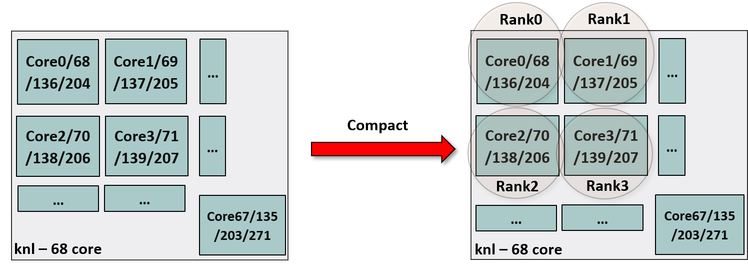
\includegraphics[width=0.75\textwidth]{Img/compact_binding.png}
 \caption{Process placement with ``hybrid'' CPU binding policy and 4 thread
          per MPI rank}
 \label{fig:compact1}
\end{figure}

\textbf{Note} --- The correct use of this environment variable mandates that \\
MV2\_CPU\_BINDING\_POLICY should be set to ``hybrid" and 
MV2\_THREADS\_PER\_PROCESS must be a positive integer. 


\textbf{spread} --- This policy ensures that no two MPI ranks get bound to 
the same physical core. Moreover, this policy will equally distribute the 
resources (physical cores and hw/threads) among the MPI processes. It also 
ensures correct bindings on some clusters that have non-trivial vendor specific mappings.

Example with 8 MPI processes and 4 OpenMP threads per process on a 68-core KNL
processor with ``spread" binding policy for threads is shown below:

\CommandBox{\$ mpirun\_rsh -hostfile hostfile -np 8 OMP\_NUM\_THREADS=4
MV2\_CPU\_BINDING\_POLICY=hybrid MV2\_THREADS\_PER\_PROCESS=4
MV2\_HYBRID\_BINDING\_POLICY=spread ./a.out}{0.9}\\

\begin{verbatim}
-------------CPU AFFINITY-------------
RANK: 0  CPU_SET:    0   1   2   3
RANK: 1  CPU_SET:    4   5   6   7
RANK: 2  CPU_SET:    8   9  10  11
RANK: 3  CPU_SET:   12  13  14  15
RANK: 4  CPU_SET:   16  17  18  19
RANK: 5  CPU_SET:   20  21  22  23
RANK: 6  CPU_SET:   24  25  26  27
RANK: 7  CPU_SET:   28  29  30  31
--------------------------------------
\end{verbatim}

This will assign one MPI rank per physical core avoiding resource contention 
caused by multiple MPI ranks getting bound to logical cores. 

\textbf{Note} --- The correct use of this environment variable mandates that  \\
MV2\_CPU\_BINDING\_POLICY should be set to ``hybrid" and 
MV2\_THREADS\_PER\_PROCESS must be a positive integer. 


\textbf{numa} --- This policy allows for MPI ranks to get bound to 
different numa domains in a round-robin manner. For example, the first process
will be bound to the first physical core of the first numa domain, the second
process on to the first physical core of the second numa domain, and so on. 
It also ensures correct bindings on some clusters that have non-trivial vendor 
specific mappings.

Example with 16 MPI processes on an AMD EPYC 7551 processor with 8 numa domains 
with is shown below: 

\CommandBox{\$ mpirun\_rsh -hostfile hosts -np 16 MV2\_CPU\_BINDING\_POLICY=hybrid 
MV2\_HYBRID\_BINDING\_POLICY=numa ./a.out}{0.9}\\

\begin{verbatim}
-------------CPU AFFINITY-------------
RANK: 0  CPU_SET:    0
RANK: 1  CPU_SET:    8
RANK: 2  CPU_SET:   16
RANK: 3  CPU_SET:   24
RANK: 4  CPU_SET:   32
RANK: 5  CPU_SET:   40
RANK: 6  CPU_SET:   48
RANK: 7  CPU_SET:   56
RANK: 8  CPU_SET:    1
RANK: 9  CPU_SET:    9
RANK:10  CPU_SET:   17
RANK:11  CPU_SET:   25
RANK:12  CPU_SET:   33
RANK:13  CPU_SET:   41
RANK:14  CPU_SET:   49
RANK:15  CPU_SET:   57
\end{verbatim}

Each MPI rank is assigned to a different NUMA domain in a round-robin manner. 
The CPU binding will be set as shown in Figure~\ref{fig:numa1}.

\begin{figure}[htbp]
 \centering
 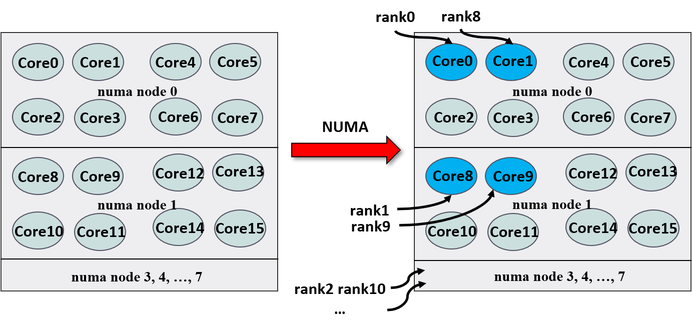
\includegraphics[width=0.75\textwidth]{Img/numa_binding.png}
 \caption{Process placement with ``hybrid'' CPU binding policy and ``NUMA``
          hybrid binding policy}
 \label{fig:numa1}
\end{figure}

\textbf{Note} --- The correct use of this environment variable mandates that  \\
MV2\_CPU\_BINDING\_POLICY should be set to ``hybrid" and 
MV2\_THREADS\_PER\_PROCESS must be a positive integer (already set by default).
Furthermore, this policy is default on AMD EPYC systems when more than two
processes are used. 


\textbf{bunch} --- assigns cores to MPI ranks in the same way as ``bunch" option
described earlier. It additionally takes care of the vendor specific 
non-trivial core mappings. Further, it also ensures that the MPI ranks are 
bound to the physical cores only. 

\textbf{scatter} --- similar to ``bunch", this also assigns cores to MPI ranks in 
``scatter" option given to MV2\_CPU\_BINDING\_POLICY. It additionally takes care 
of vendor specific non-trivial core mappings. It also 
ensures that the MPI ranks are only bound to the physical cores only.

\textbf{Note} --- ``bunch" and ``scatter" options for MV2\_HYBRID\_BINDING\_POLICY are 
recommended to be used as a solution to vendor specific non-trivial mapping issues. These 
should be considered an alternate to ``bunch" or ``scatter" given to CPU\_BINDING\_POLICY.

\subsection{Running with Hot-Spot and Congestion Avoidance}
\label{def:mv2-hsam}
MVAPICH2 supports hot-spot and congestion avoidance using InfiniBand
multi-pathing mechanism. This support is available for MPI applications
using OFA-IB-CH3 interface.

To enable this functionality, a run-time variable,
MV2\_USE\_HSAM (Section~\ref{def:mv2-use-hsam})
can be enabled, as shown in the following example:
\\
\CommandBox{\$ mpirun\_rsh -np 2 n0 n1 MV2\_USE\_HSAM=1 ./cpi}{0.9} \\
or \\
\CommandBox{\$ mpiexec -n 2 -hosts n0,n1 -env MV2\_USE\_HSAM 1 ./cpi}{0.9} \\

This functionality automatically defines the number of paths for
hot-spot avoidance. Alternatively, the maximum number of paths to be
used between a pair of processes can be defined by using a run-time
variable MV2\_NUM\_QP\_PER\_PORT (Section~\ref{def:num-qp-per-port}).

We expect this functionality to show benefits in the presence of
at least partially non-overlapping paths in the network. OpenSM, the subnet manager
distributed with OpenFabrics supports LMC mechanism, which can be used
to create multiple paths:

\CommandBox{\$ opensm -l4}{0.9} \\

will start the subnet manager with LMC value to four, creating sixteen
paths between every pair of nodes.

\subsection{Running on Clusters with NVIDIA GPU Accelerators}
\label{def:mv2-gpu}

MVAPICH2 CH3-based interface supports MPI communication using NVIDIA GPU device memory
with CUDA versions 4.0 or later. This feature removes the need for the application developer
to explicitly move the data from device memory to host memory before using MPI for communication.
The new support allows direct MPI communication from device memory to device memory,
device memory to host memory and host memory to device memory. It also supports point-to-point and
collective communication using contiguous and non-contiguous MPI datatypes. It takes advantage of CUDA IPC
for intra-node GPU-GPU communication (with CUDA 4.1).\\
\\
For example, without CUDA support in the MPI library, a typical user might be using
the following sequence of commands to move data from a device memory
to another device memory.\\
\\
\textit{\ldots\\
cudaMemcpy(host\_buf, device\_buf, size, cudaMemcpyDeviceToDevice);\\
MPI\_Isend(host\_buf, size, MPI\_CHAR, 1, 100, MPI\_COMM\_WORLD, req);\\
\ldots\\}
\\
With the support provided in MVAPICH2 and support of CUDA 4.0 (and later),
the user can achieve the same data movement operation by explicitly specifying MPI calls on device memory. \\
\textit{\ldots\\
MPI\_Isend(device\_buf, size, MPI\_CHAR, 1, 100, MPI\_COMM\_WORLD, req);\\
\ldots\\}

This support can be enabled by configuring MVAPICH2 with \texttt{--enable-cuda} and
setting the environment variable MV2\_USE\_CUDA (~\ref{def:use-cuda}) to 1
during runtime.

To minimize communication overhead, MVAPICH2 divides copies between device and
host into chunks.  This can be better tuned for internode transfers with a
runtime environment variable MV2\_CUDA\_BLOCK\_SIZE
(~\ref{def:cuda-block-size}).  The default chunk size is 64K (65536). However,
higher values of this parameter, such as 256K (262144) and 512K (524288), might
deliver better performance if the MPI application uses large messages. The
optimal value for this parameter depends on several other factors such as
InfiniBand network/adapter speed, GPU adapter characteristics, platform
characteristics (processor and memory speed) and amount of memory to be
dedicated to the MPI library with GPU support. For different platforms and MPI
applications, the users are encouraged to try out different values for this
parameter to get best performance.

MVAPICH2 takes advantage of tunable two-dimensional CUDA kernel for
packing/unpacking data when MPI vector datatype is used in communication
involving GPU memory. The CUDA thread block size and dimensions are
automatically tuned based on the dimensions of the vector. Users can also
control the number of CUDA threads per block using the runtime parameter:
MV2\_CUDA\_KERNEL\_VECTOR\_TIDBLK\_SIZE (default value is 1024)
(~\ref{def:cuda-kernel-vector-threadblock}).  They can adjust the number of
threads operating on each data block of the vector using \\
MV2\_CUDA\_KERNEL\_VECTOR\_YSIZE (tuned based on vector size)
(~\ref{def:cuda-kernel-vector-ysize}).

%For intranode transfers, the chunk size is
%controlled by the runtime environment variable MV2\_SMP\_SEND\_BUF\_SIZE and
%its default value is 128K (131072) when CUDA support is enabled. Other
%recommended values for this variable are 64K (65536) and 256K (262144). Users
%have to note that the parameter MV2\_SMP\_SEND\_BUF\_SIZE will also impact
%host-to-host intranode communication in which case smaller chunk sizes (8K or
%16K) deliver better performance.
%MVAPICH2 uses network loopback for intra node communication when
%MV2\_USE\_CUDA(~\ref{def:use-cuda}) is enabled. In order to use
%MVAPICH2 NVIDIA GPU features on stand alone multi-core GPU nodes that are
%not equipped with InfiniBand adapters, users need to enable shared memory through the
%following run time environment variables: MV2\_USE\_SHARED\_MEM=1 MV2\_SMP\_SEND\_BUF\_SIZE=262144.
%The parameter MV2\_SMP\_SEND\_BUF\_SIZE(~\ref{def:smp-send-buf-size})
%controls the size of copies used in large message shared memory communication.
%Users can better tune based on the requirement. Some suggested values
%are 65536, 131072 or 524288.

\paragraph{GPU Affinity:}

When multiple GPUs are present on a node, users might want to set the
MPI process affinity to a particular GPU using cuda calls like cudaSetDevice().
This can be done after MPI\_Init based on MPI rank of the process or before
MPI\_Init using the local rank of a process obtained from an environment variable
MV2\_COMM\_WORLD\_LOCAL\_RANK.

%But MVAPICH2
%performs some cuda operations like buffer registration and others during MPI\_Init
%which result in default context creation. Hence, setting GPU Affinity after MPI\_Init
%could create issues due to the context switch. To avoid this, MVAPICH2 provides an
%environment variable called MV2\_COMM\_WORLD\_LOCAL\_RANK to get the local rank of a
%process on its node before MPI\_Init is called. This local rank information can be
%used to set GPU affinity before MPI\_Init is called as given in the following
%code example
%\\
%\textit{\ldots\\
%....\\
%int local\_rank = atoi(getenv("MV2\_COMM\_WORLD\_LOCAL\_RANK"));\\
%cudaSetDevice(local\_rank \% num\_devices);\\
%...\\
%MPI\_Init() \\
%...\\
%\ldots\\}
%\\
%This local rank information can also be used in wrapper scripts to set cpu and memory
%affinity on nodes with NUMA.

\subsection{MPIRUN\_RSH compatibility with MPIEXEC}
There is now a front end to mpirun\_rsh that aims for compatibility with mpiexec
usage as recommended by the MPI standard.  This front end is can be used by
calling mpiexec.mpirun\_rsh.

The main differences between this and mpirun\_rsh is that this front end
doesn't require you to specify hosts or environment variables on the command
line.  Also, the host file options is -f as opposed to -hostfile.

\noindent Run 4 instances of CPI on localhost:

\CommandBox{\$ mpiexec.mpirun\_rsh -n 4 ./cpi}{0.7}

\noindent Run 4 instances of CPI on the nodes specified by hostfile:

\CommandBox{\$ mpiexec.mpirun\_rsh -n 4 -f hostfile ./cpi}{0.7}

\subsubsection{Interaction with SLURM}
If the hostfile isn't given and mpiexec.mpirun\_rsh finds the appropriate slurm
environment variables set, mpiexec will use these to determine which nodes the
applications should be launched on.

Please note that processes are assigned in a block fashion by slurm so all the processes will run on the same node if possible.

\noindent Run 4 instances of CPI on up to 4 different nodes (but maybe only 1)
allocated by ``salloc'':

\CommandBox{\$ salloc -N 4\\
    \$ mpiexec.mpirun\_rsh -n 4 ./cpi}{0.7}

\noindent Same thing as above but only allocating the minimum number of nodes
needed to run 4 tasks:

\CommandBox{\$ salloc -n 4\\
    \$ mpiexec.mpirun\_rsh ./cpi}{0.7}

\noindent Run 4 instances of CPI on 4 different nodes allocated by ``salloc'':

\CommandBox{\$ salloc -N 4 --ntasks-per-node=1\\
    \$ mpiexec.mpirun\_rsh -n 4 ./cpi}{0.7}

\subsubsection{Interaction with PBS}
If the hostfile isn't given and mpiexec.mpirun\_rsh finds the PBS\_NODEFILE
environment variable set, mpiexec will use this to locate the host file.

\subsection{Running with Intel Trace Analyzer and Collector}

MVAPICH2 supports compiling and running MPI applications with Intel Trace Analyzer and Collector (ITAC), so that the MPI calls in an execution can be traced, and the logs can be used for functionality or performance analysis. The following steps need to be done to make an MPI application work with ITAC.

\begin{itemize}
\item Export the environment variables of ITAC. You can either export the entire set of ITAC variables for your architecture by script:

\CommandBox{\$ source /opt/intel/itac/8.1.4/intel64/bin/itacvars.sh}{0.7}

or simply export the only variable of VTune root that needed by MVAPICH2:

\CommandBox{\$ export VT\_ROOT=/opt/intel/itac/8.1.4}{0.7}

\item Compile your application using \texttt{mpicc}, \texttt{mpifort} or other compiling commands with the ``\texttt{-itac}'' option. For example:

\CommandBox{\$ mpicc -itac -o cpi cpi.c}{0.7}

If configure/Makefile or other building scripts are employed, you should append ``\texttt{-itac}'' to the compiling and linking options such as ``\texttt{CFLAGS}''. For example:

\CommandBox{\$ ./configure CC=mpicc CFLAGS=-itac \&\& make}{0.7}

\item Run the created binary with an MPI launcher in the normal way. After execution, the ITAC prompt information will be printed on stderr, and some trace files will be created in current directory.

\item Launch the GUI tool of ITAC on a desktop environment or through X11 forwarding from the server, load the trace file with the ``\texttt{.stf}'' suffix, and the MPI calls within that execution can be visualized and analyzed.
\end{itemize}

The advanced usage of ITAC can be found at: \href{https://software.intel.com/en-us/intel-trace-analyzer}{https://software.intel.com/en-us/intel-trace-analyzer}.


\subsection{Running with MCDRAM support on Intel Knights Landing (KNL) processor}
\label{sec:mcdram}

This section describes the procedure to take advantage of the High Bandwidth
Memory (MCDRAM) available with the Intel Knights Landing processor. The method
discussed here is basic and does not require modifications to the user
application or MPI library.

%\subsubsection{
\noindent \textbf{Allocating Memory on MCDRAM}

\noindent In order to do all the memory allocations including application
buffers and/or internal buffers of MVAPICH2, one can use the \textit{numactl}
system call. This is beneficial when KNL is configured in Flat/Hybrid mode where
MCDRAM can be viewed as separate NUMA node.

\noindent \textit{Step 1}: Verify that KNL is configured in Flat/Hybrid mode.
One can execute the \textit{numactl -H} command to verify this. A sample output
is also given below.
As can be seen from the sample output, when KNL is in Flat-mode NUMA node 0
consists of all the processor cores and DDR memory ( approximately 96GB in
size). NUMA node 1 consists of only the MCDRAM (approximately 16GB in size).

\CommandBox{\$ numactl -H}{0.7}

\begin{verbatim}
	[hashmij@knl1 pt2pt]$ numactl -H
	available: 2 nodes (0-1)
	node 0 cpus: 0 1 2 3 4 5 6 7 8 9 10 11 12 13 14 15 16 17 18 19 20 21 22
	23 24 25 26 27 28 29 30 31 32 33 34 35 36 37 38 39 40 41 42 43 44 45 46
	47 48 49 50 51 52 53 54 55 56 57 58 59 60 61 62 63 64 65 66 67 68 69 70
	71 72 73 74 75 76 77 78 79 80 81 82 83 84 85 86 87 88 89 90 91 92 93 94
	95 96 97 98 99 100 101 102 103 104 105 106 107 108 109 110 111 112 113
	114 115 116 117 118 119 120 121 122 123 124 125 126 127 128 129 130 131
	132 133 134 135 136 137 138 139 140 141 142 143 144 145 146 147 148 149
	150 151 152 153 154 155 156 157 158 159 160 161 162 163 164 165 166 167
	168 169 170 171 172 173 174 175 176 177 178 179 180 181 182 183 184 185
	186 187 188 189 190 191 192 193 194 195 196 197 198 199 200 201 202 203
	204 205 206 207 208 209 210 211 212 213 214 215 216 217 218 219 220 221
	222 223 224 225 226 227 228 229 230 231 232 233 234 235 236 237 238 239
	240 241 242 243 244 245 246 247 248 249 250 251 252 253 254 255 256 257
	258 259 260 261 262 263 264 265 266 267 268 269 270 271
	node 0 size: 98200 MB
	node 0 free: 94215 MB
	node 1 cpus:
	node 1 size: 16384 MB
	node 1 free: 15929 MB
	node distances:
	node   0   1
	  0:  10  31
	  1:  31  10 
\end{verbatim}
   
\noindent \textit{Step 2}: Executing applications to take advantage of MCDRAM.

All memory allocations made by the application as well as MVAPICH2 can be
redirected to MCDRAM by prepending \textit{numactl --membind
$<$MCDRAM\_numa\_node$>$} to the job invocation. An example of the same is given
below.

\CommandBox{\$ numactl --membind 1 mpirun\_rsh -np 2 -hostfile hosts osu\_latency}{0.7} \\

%\subsubsection{
\noindent \textbf{Viewing MCDRAM Allocations}

\noindent To verify that the allocations are indeed being done on the MCDRAM,
the \textit{numastat -p $<$pid$>$} command can be used where ``pid'' refers to the
process ID of one of the application processes. An example of the same is given
below.

Note that the pages are not allocated until the memory is actually ``touched''
by the application and/or the MVAPICH2 MPI library. Thus, `\texttt{numastat}'
will only report a difference in the amount of memory after the memory is
touched.

\CommandBox{\$ numastat -p 21356}{0.7}
\noindent\begin{verbatim} 
Per-node process memory usage (in MBs) for PID 95610 (osu_latency)
   		                       Node 0          Node 1           Total
       		          --------------- --------------- ---------------
	Huge                         0.00            0.00            0.00
	Heap                         0.00            1.40            1.40
	Stack                        0.00            0.08            0.08
	Private                      3.11           73.89           77.00
	----------------  --------------- --------------- ---------------
	Total                        3.11           75.37           78.48  
\end{verbatim}   
\subsection{Running Collectives with Hardware based SHArP support}
\label{subsec:coll-sharp}

In MVAPICH2, support for SHArP-based collectives has been enabled for MPI
applications running over OFA-IB-CH3 interface. Currently, this support is
available for the following collective operations:

\begin{itemize}
		\item{MPI\_Allreduce}
\end{itemize}

This feature is disabled by default at configuration time. To use this feature, you need to use
\texttt{--enable-sharp} configuration option and specify the path to SHArP installation
location by adding the paths to LDFLAGS and CFLAGS. Also, \texttt{-lsharp} and
\texttt{-lsharp\_coll} flags must be added to LDFLAGS. See the example below.

\begin{verbatim}
./configure --enable-sharp LDFLAGS="-Wl,-rpath,/opt/hpcx/1.8/sharp/lib
-L/opt/hpcx/1.8/sharp/lib -lsharp -lsharp_coll" 
CFLAGS="-I/opt/hpcx/1.8/sharp/include/sharp" 
\end{verbatim}

Please note that SHArP library is a part of HPCX Software Toolkit and the
network must be equipped with Mellanox Switch-IB2. Currently, MVAPICH2 supports
SHArP library of HPCX v1.7 and v1.8.

Note that the various SHArP related daemons (SHArP Aggregation Manager -
\textit{sharpam} and the local SHArP daemon - \textit{sharpd} must be installed,
setup and running for SHArP support in MVAPICH2 to work properly.  This can be
verified by running the \texttt{sharp\_hello} program available in the ``bin''
sub-folder of the SHArP installation directory.

This feature is turned off by default at runtime and can be turned on at runtime by using parameter
MV2\_ENABLE\_SHARP=1 (~\ref{def:enable-sharp}). Collective tuning has been done
to ensure the best performance. 

When using HPCX v1.7, we recommend setting SHARP\_COLL\_ENABLE\_GROUP\_TRIM=0
environment variable. Note that if you are using \texttt{mpirun\_rsh} you need
to add \texttt{-export} option to make sure that environment variable is
exported correctly.
This environment variable is a part of SHArP library. 
Please refer to SHArP
\href{http://www.mellanox.com/related-docs/prod_acceleration_software/Mellanox_SHARP_SW_Deployment_Guide_v1.7.1.pdf}{userguide} for more information.
